\documentclass[conference]{IEEEtran}

% Core Packages
\usepackage{amsmath,amssymb,amsfonts}
\usepackage{booktabs}
\usepackage{graphicx}
\usepackage{cite}
\usepackage{url}
\usepackage{microtype}
\usepackage[hidelinks]{hyperref}

% IEEEtran bibliography settings
\def\BibTeX{{\rm B\kern-.05em{\sc i\kern-.025em b}\kern-.08em
    T\kern-.1667em\lower.7ex\hbox{E}\kern-.125emX}}

\begin{document}

\title{TrustEval: An Empirical Study of Ensemble Reliability in Small Open-Weight LLM Safety Judges}

% Author details placeholder (strictly anonymized / unconfirmed)
\author{
    \IEEEauthorblockN{[Author Names Redacted for Blind Review / Placeholder]}
    \IEEEauthorblockA{\textit{[Department Placeholder]} \\
    \textit{[Institution / Organization Placeholder]} \\
    [City, Country Placeholder] \\
    Email: [placeholder@institution.edu]}
}

\maketitle

\begin{abstract}
Evaluating the safety of large language model (LLM) conversations increasingly relies on automated LLM-as-a-judge architectures, yet deploying massive proprietary models introduces significant cloud dependency, latency, and data confidentiality constraints. Compact open-weight language models ($<2\text{B}$ parameters) offer an attractive on-premises alternative executable on commodity CPU hardware, but their reliability, probability calibration, and alignment with nuanced human safety consensus remain fundamentally uncharacterized. In this study, we present \textbf{TrustEval}, an empirical investigation evaluating sub-2B open-weight safety judges and their ensembling characteristics against continuous human consensus. Using a fixed sample of $N=50$ multi-turn adversarial dialogues from Google DICES-350, annotated by 104 retained crowd raters per conversation ($5,200$ total ratings), we extract conditional next-token unsafe probabilities from \texttt{Qwen2.5-0.5B-Instruct} and \texttt{SmolLM2-1.7B-Instruct} using standardized prompting in native chat templates on commodity CPUs ($<1.2\text{ GB}$ RSS). 

Our findings reveal pronounced single-judge polarization: Qwen acts as an aggressive, risk-averse detector ($\bar{P}=0.7509$, $\text{MAE}=0.4152$) with strong ranking sensitivity ($\text{AUROC}=0.7529$), whereas SmolLM2 exhibits extreme variance compression ($\bar{P}=0.2531$, $\text{MAE}=0.1734$), anchoring adjacent to benchmark prevalence. An equal-weight two-judge ensemble reduces Qwen's MAE by $40.6\%$ ($0.2464$) and Soft MSE by $67.6\%$ ($0.0713$), capturing the highest linear and rank correlation with human consensus among the evaluated models ($r=0.4992$, $\rho=0.5903$) while preserving majority discrimination ($\text{AUROC}=0.7517$). However, the ensemble does not universally dominate: SmolLM2 achieves lower sample MAE, a held-out prevalence baseline achieves lower Soft MSE ($0.0602$), and the ensemble remains systematically overpredicting ($\text{ECE}_{10}=0.1639$). Furthermore, inter-judge disagreement exhibits an exploratory association with ensemble error, showing nominal in-sample linear significance ($r=0.3125, p=0.0271$; nested OLS incremental $p=0.0214$) but non-significant monotonic rank ordering ($\rho=0.2302, p=0.1078$), with low disagreement failing to guarantee correctness due to potential shared blind spots. These results demonstrate that while compact ensembling offers measurable reliability gains, it represents a nuanced trade-off rather than a turnkey solution, underscoring that sub-2B judges are suitable for exploratory research triage rather than autonomous safety certification.

\end{abstract}

\begin{IEEEkeywords}
Large language models, LLM-as-a-judge, safety evaluation, ensemble reliability, calibration, open-weight language models.
\end{IEEEkeywords}

% Modular Sections
\section{Introduction}
\label{sec:introduction}

As conversational Large Language Models (LLMs) are increasingly integrated into customer support, clinical workflows, legal analysis, and autonomous agent loops, verifying that chatbot outputs adhere to safety standards is a paramount operational requirement. While human moderation remains the authoritative gold standard, manual auditing cannot scale to the throughput demands of continuous production monitoring. Consequently, automated evaluation pipelines—popularized under the \textit{LLM-as-a-judge} paradigm~\cite{chiang2023vicuna,zheng2023judging,wang2023pandalm}—are widely adopted to evaluate conversational responses and detect safety violations~\cite{zhang2024safetybench,mazeika2024harmbench}.

Standard LLM-as-a-judge deployments rely almost exclusively on commercial cloud-hosted frontier models or large open-weight clusters ($70\text{B}+$ parameters)~\cite{touvron2023llama,tan2025judgebench,bavaresco2025llms}. While effective for high-level capabilities, this centralized cloud paradigm introduces persistent operational and governance challenges:
\begin{enumerate}
    \item \textbf{Data Privacy and Regulatory Governance:} While lawful cloud processing can be structured through formal Data Processing Agreements (DPAs) and institutional safeguards, transmitting user conversations to external commercial inference APIs introduces ongoing compliance management under data protection frameworks such as GDPR and HIPAA~\cite{debenedetti2024evading}. Local model inference avoids sending evaluated dialogue data to third-party model APIs, ensuring conversational data remains within internal boundaries, though institutional regulatory compliance ultimately depends on broader system-level security controls.
    \item \textbf{Economic and Throughput Overhead:} Sustained offline evaluation of high-volume conversational logs incurs recurring API token expenditures and operational exposure to rate-limiting bottlenecks.
    \item \textbf{Logit Obfuscation and Uncertainty Blindness:} Commercial model APIs frequently restrict or withhold raw next-token logit distributions, preventing downstream systems from extracting continuous probability estimates or evaluating predictive confidence.
\end{enumerate}

These operational constraints motivate investigating \textit{small open-weight language models} (SLMs) with fewer than 2 billion parameters~\cite{yang2024qwen25,allal2025smollm2} as localized safety evaluators. Sub-2B models can execute deterministically on commodity x86 CPUs within bounded memory footprints ($\le 8\text{ GB}$ system RAM, peak resident set size $< 1.2\text{ GB}$), enabling self-contained on-premises evaluation without requiring dedicated GPU acceleration.

\begin{figure}[t]
    \centering
    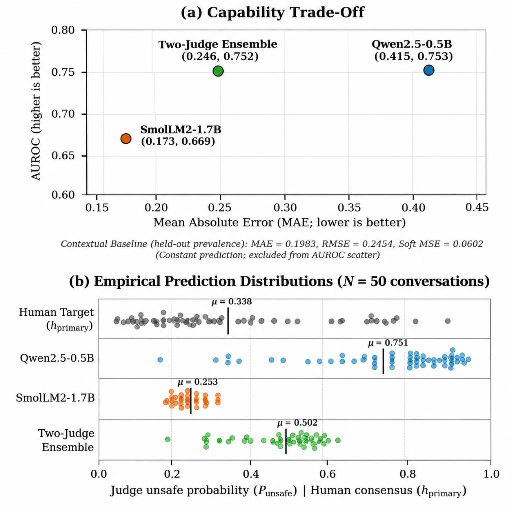
\includegraphics[width=\columnwidth]{figures/fig1_tradeoff.pdf}
    \caption{Evaluator polarization and the ensembling trade-off frontier on an exploratory sample of $N=50$ multi-turn adversarial conversations from Google DICES-350. (a) Capability trade-off plane: Mean Absolute Error (MAE, lower is better) versus majority-consensus discrimination ($\text{AUROC}$, higher is better). Qwen2.5-0.5B achieves high ranking sensitivity ($\text{AUROC} = 0.7529$, Spearman $\rho = 0.5680$) but high error ($\text{MAE} = 0.4152$). SmolLM2-1.7B achieves the lowest judge MAE ($0.1734$) but compressed ranking acuity ($\text{AUROC} = 0.6690, \rho = 0.3929$). The Two-Judge Ensemble provides an empirical compromise, cutting Qwen's MAE by $40.6\%$ while capturing the highest rank correlation ($\rho = \mathbf{0.5903}$) and preserving AUROC ($0.7517$). The ensemble does not universally dominate: SmolLM2 achieves lower sample MAE, and a 5-fold held-out prevalence baseline achieves lower squared error ($\text{Soft MSE} = 0.0602$). (b) Single-model prediction distributions ($N=50$) demonstrating Qwen's positive hazard bias ($\mu = 0.751$) and SmolLM2's variance collapse ($\sigma = 0.039$) clustered near dataset prevalence ($0.338$).}
    \label{fig:tradeoff}
\end{figure}

However, deploying compact models as autonomous safety evaluators introduces documented reliability risks. Constrained parameter capacities make small models prone to inductive biases, severe probability miscalibration, and vulnerability to subtle phrasing shifts~\cite{tan2025judgebench,schwinn2026coin}. Recent audits demonstrate that automated judges can collapse toward chance-level accuracy when evaluating adversarial distributions~\cite{schwinn2026coin}. Furthermore, existing benchmarks predominantly collapse multi-rater evaluations into binary majority consensus, obscuring the nuanced distribution of human judgments~\cite{aroyo2023dices,davani2022dealing,rottger2022two}.

In classical machine learning, ensembling diverse model checkpoints is a recognized approach to mitigate individual inductive biases and improve predictive reliability~\cite{lakshminarayanan2017simple,ovadia2019can}. While multi-agent jury architectures have been explored for frontier models~\cite{verga2024replacing,qian2026who}, whether an ensemble of \textit{heterogeneous sub-2B open-weight models} running locally on commodity CPUs can reliably approximate continuous human safety consensus remains fundamentally uncharacterized.

To investigate this question, this paper presents \textbf{TrustEval}, an empirical study evaluating the representational accuracy, ranking discrimination, calibration behaviour, and error-uncertainty dynamics of small open-weight LLM safety judges. We analyze an equal-weight ensemble of two structurally distinct sub-2B models—\texttt{Qwen2.5-0.5B-Instruct} (0.49B parameters) and \texttt{SmolLM2-1.7B-Instruct} (1.71B parameters)—evaluated on multi-turn conversational dialogues drawn from the Google DICES-350 benchmark~\cite{aroyo2023dices}. Each conversation in DICES-350 contains ratings from 104 retained human crowd annotators, allowing us to evaluate models directly against continuous human consensus proportions ($h_{\text{primary}} \in [0, 1]$). Furthermore, we examine whether inter-judge disagreement ($\Delta = |P_{\text{qwen}} - P_{\text{smol}}|$) functions as an exploratory candidate correlate for ensemble evaluation error.

As previewed in Fig.~\ref{fig:tradeoff}, our empirical investigation uncovers a pronounced trade-off between constituent judges: Qwen2.5-0.5B exhibits strong discriminative hazard ordering alongside severe positive prediction bias, whereas SmolLM2-1.7B achieves low absolute error through conservative prevalence anchoring at the cost of compressed prediction variance. An unweighted ensemble negotiates this trade-off frontier, moderating prediction error relative to Qwen while improving rank correlation over both individual judges.

\subsection{Research Questions}
\label{sec:rqs}

This paper addresses three research questions established in our pre-registered experimental protocol:
\begin{itemize}
    \item \textbf{RQ1 (Representation and Point Error):} Can small open-weight LLMs ($\le 1.7\text{B}$ parameters) running on commodity CPU hardware approximate continuous human safety consensus ($h \in [0, 1]$), and how does an equal-weight ensemble compare against individual constituent judges and naive prevalence baselines in point error (MAE, RMSE, Soft MSE) and decile calibration (Soft ECE-10)?
    \item \textbf{RQ2 (Discriminative Ranking Capacity):} How do individual small judges and their ensemble perform in ranking conversational hazard relative to human consensus (Pearson $r$, Spearman $\rho$, AUROC), and does ensembling preserve discriminative sensitivity while tempering single-model prediction bias?
    \item \textbf{RQ3 (Disagreement as a Candidate Error Correlate):} Does inter-judge disagreement ($\Delta$) between diverse small judges provide a statistically defensible, cross-validated candidate surrogate signal for ensemble evaluation error, predicting uncertainty beyond response character length and ensemble predicted unsafe probability?
\end{itemize}

\subsection{Summary of Contributions}
\label{sec:contributions}

The primary contributions of this paper are:
\begin{enumerate}
    \item \textbf{Empirical Audit of Sub-2B Judges on Continuous Human Consensus:} We conduct an empirical evaluation of sub-2B open-weight LLMs tasked with predicting continuous human safety consensus ($h_{\text{primary}} \in [0, 1]$) derived from 104 crowd annotators per item ($5,200$ total ratings) across 50 multi-turn dialogues sampled from Google DICES-350.
    \item \textbf{Characterization of Single-Judge Trade-Offs:} We identify a clear divergence in small-model evaluation behaviour: Qwen2.5-0.5B achieves high discriminative ordering ($\text{AUROC} = 0.7529, \text{Spearman } \rho = 0.5680$) but exhibits substantial positive prediction bias ($\mu = 0.7513$ vs. human mean $0.3381$) and miscalibration ($\text{ECE-10} = 0.4128$). Conversely, SmolLM2-1.7B achieves the lowest observed sample MAE ($0.1734$) via variance compression ($\sigma = 0.0388$) near sample prevalence, with modest binary discrimination ($\text{AUROC} = 0.6690$) and a positive rank correlation ($\rho = 0.3929, p = 0.0048$). We document that SmolLM2's MAE advantage is test-sensitive (statistically significant under a paired $t$-test and sign test, but non-significant under a Wilcoxon signed-rank test after family-wise Holm adjustment; $W = 427.0, p_{\text{adj}} = 0.0843$).
    \item \textbf{Empirical Pareto Expansion via Ensembling:} We show that an equal-weight two-judge ensemble synthesizes these complementary behaviours, cutting Qwen's MAE by $40.6\%$ (to $0.2464$, $p = 1.04 \times 10^{-7}$) and Soft MSE by $67.6\%$ ($p = 2.85 \times 10^{-9}$) while maintaining comparable AUROC ($0.7517$) and attaining the highest rank correlation ($\rho = \mathbf{0.5903}$, $p = 6.43 \times 10^{-6}$) and linear correlation ($r = \mathbf{0.4992}$, $p = 0.0002$) across all evaluators. We emphasize that ensembling represents an observed empirical trade-off rather than universal superiority: it does not outperform SmolLM2 in point MAE, and it moderates rather than completely eliminates prediction bias.
    \item \textbf{Empirical Baseline Reality Check:} We transparently document that in squared error (Soft MSE), a naive 5-fold held-out prevalence baseline achieves the lowest overall error ($0.0602$), outperforming all evaluated models including the ensemble ($0.0713$), illustrating the challenge small models encounter under quadratic loss when competing against sample prevalence.
    \item \textbf{Exploratory Analysis of Disagreement as an Error Correlate:} We show that inter-judge disagreement ($\Delta$) exhibits a nominally significant positive association with ensemble absolute error ($r = 0.3125, p = 0.0271$). In nested in-sample OLS regression controlling for response length and ensemble prediction, adding $\Delta$ yields a statistically significant incremental variance gain ($F(1, 46) = 5.676, p = 0.0214$) and an out-of-fold descriptive gain of $\Delta R^2_{\text{OOF}} = +0.0805$ across 5-fold cross-validation. We rigorously qualify disagreement as a preliminary candidate correlate rather than a validated uncertainty metric.
    \item \textbf{Practical Edge-Inference Profiling:} We demonstrate that deterministic next-token logit scoring executes locally on commodity x86 laptop CPUs within a bounded envelope ($< 1.2\text{ GB}$ peak resident set size), confirming the computational feasibility of decentralized safety auditing.
\end{enumerate}

\subsection{Paper Roadmap}
\label{sec:roadmap}

The remainder of this paper is organized as follows: Section~\ref{sec:related_work} synthesizes related literature across LLM judges, safety benchmarks, calibration, and ensemble uncertainty. Section~\ref{sec:dataset_ground_truth} details the DICES-350 benchmark, crowd annotator filtering, and continuous target formulation. Section~\ref{sec:methodology_experimental_setup} outlines model architectures, native ChatML prompt serialization, and logit scoring protocols. Section~\ref{sec:results} presents empirical findings across point error, calibration, discriminative ranking, and inter-judge disagreement modeling (Subsection~\ref{subsec:disagreement_analysis}). Section~\ref{sec:discussion} discusses operational trade-offs, calibration nuances, and edge deployment implications. Section~\ref{sec:limitations_ethics} details empirical limitations and responsible AI considerations. Finally, Section~\ref{sec:conclusion} concludes the paper with future research directions.

\section{Related Work}
\label{sec:related_work}

\subsection{Automated LLM-as-a-Judge Paradigms}
\label{sec:rel_llm_judge}

The concept of leveraging instruction-tuned language models as automated evaluators emerged alongside conversational assistants~\cite{chiang2023vicuna} and was formalized by Zheng et al.~\cite{zheng2023judging} through MT-Bench and Chatbot Arena. Subsequent frameworks, such as PandaLM~\cite{wang2023pandalm}, demonstrated that LLMs could evaluate instruction-following quality with moderate human agreement. However, as automated judging expanded into high-stakes safety and capability evaluation, recent literature has exposed fundamental vulnerabilities in the LLM-as-a-judge paradigm.

Tan et al.~\cite{tan2025judgebench} introduced JudgeBench, revealing that commercial judges frequently rely on spurious heuristics, including length bias, position bias, and self-enhancement bias (favoring their own generated completions). In an extensive empirical evaluation across 20 distinct NLP evaluation tasks, Bavaresco et al.~\cite{bavaresco2025llms} established that while frontier models correlate moderately with human judgments on simple lexical tasks, their alignment degrades significantly on complex subjective tasks requiring nuanced pragmatic interpretation. Most critically, Schwinn et al.~\cite{schwinn2026coin} demonstrated that state-of-the-art LLM judges fail catastrophically when evaluating adversarial robustness and jailbreak prompts, with classification performance collapsing toward random chance (``a coin flip'') due to semantic perturbation sensitivity. While Schwinn et al. audit binary robustness classifications across frontier and medium-scale models, TrustEval investigates whether an ensemble of sub-2B models can approximate continuous human safety consensus on conversational dialogues, and whether inter-judge disagreement correlates with evaluation error.

\subsection{Safety Benchmarks and Crowdsourced Disagreement}
\label{sec:rel_safety_disagreement}

Automated safety evaluation has been driven by standardized benchmarks such as SafetyBench~\cite{zhang2024safetybench} and HarmBench~\cite{mazeika2024harmbench}. However, conventional benchmarks universally aggregate multi-annotator ratings into single majority-vote binary labels ($0$ or $1$), treating annotator disagreement as unstructured label noise.

A growing body of human-centered machine learning literature argues that human disagreement is not mere noise, but a reflection of legitimate sociodemographic, cultural, and ethical divergence~\cite{basile2021we,davani2022dealing,rottger2022two}. Gordon et al.~\cite{gordon2021disagreement} introduced disagreement deconvolution to align model predictions with high-disagreement contexts, while Jury Learning~\cite{gordon2022jury} explicitly architectures classifiers to model diverse annotator compositions. In conversational safety, Aroyo et al.~\cite{aroyo2023dices} introduced the Diversity in Conversational AI Evaluation for Safety (DICES) benchmark, deliberately capturing granular crowd judgments across diverse demographic strata. In TrustEval, rather than binarizing annotations into an artificial consensus, we formulate our target as the continuous empirical hazard rate ($h_{\text{primary}} \in [0, 1]$) across 104 verified crowd raters per dialogue.

\subsection{Model Calibration, Soft Labels, and Expected Calibration Error}
\label{sec:rel_calibration}

In classification systems, a model is well-calibrated if its predicted probability reflects the true long-run empirical frequency of the event~\cite{brier1950verification}. Guo et al.~\cite{guo2017calibration} established that modern deep neural networks, despite achieving superior classification accuracy, suffer from severe miscalibration and overconfidence. Evaluating calibration typically relies on Expected Calibration Error (ECE) and reliability diagrams, which partition predictions into equal-width bins and compare mean confidence against empirical accuracy.

While standard ECE assumes hard binary labels ($y \in \{0, 1\}$), evaluating models against multi-annotator distributions requires extending calibration to continuous soft targets ($h \in [0, 1]$). Under dataset shift and challenging dialogue conditions, predictive probabilities frequently drift far from empirical targets~\cite{ovadia2019can}. In TrustEval, we compute decile Soft ECE-10 over continuous human targets, revealing structural calibration anomalies—including severe overprediction in Qwen2.5-0.5B and degenerate single-bin artifacts in prevalence baselines.

\subsection{Multi-Model Ensembles and Disagreement in LLMs}
\label{sec:rel_ensembles}

Deep ensembling, pioneered by Lakshminarayanan et al.~\cite{lakshminarayanan2017simple}, is recognized as an effective and scalable approach for predictive uncertainty estimation and out-of-distribution robustness. In language modeling, uncertainty quantification has largely focused on semantic entropy across stochastic generations from a single checkpoint~\cite{kuhn2023semantic,malinin2018predictive}.

More recently, multi-model panels have been adapted to evaluation. Verga et al.~\cite{verga2024replacing} demonstrated that replacing individual judges with panels of diverse LLMs mitigates individual model biases on instruction-following benchmarks. Qian et al.~\cite{qian2026who} developed LLM-as-a-Jury, combining multiple frontier judges to improve comparative assessment on MT-Bench. Concurrently, theoretical frameworks by Li~\cite{li2026calibrate} and Feng et al.~\cite{feng2026noisy} demonstrated that pooling predictions from imperfect, noisy judges can yield statistically consistent population estimates when individual error distributions are properly accounted for. Zhang et al.~\cite{zhang2026can} explored multi-judge ensembles for bias calibration across capability dimensions.

In the domain of small language models, Laddha et al.~\cite{laddha2026slmjury} introduced SLMJury, investigating whether panels of compact models (0.6B to 14B parameters) can match frontier model quality on discrete preference benchmarks. However, SLMJury focuses on discrete voting and generative deliberation for general NLP tasks. TrustEval uniquely explores whether an ensemble of sub-2B off-the-shelf models executing on consumer CPU hardware can approximate continuous multi-annotator safety consensus, and whether the inter-judge disagreement ($\Delta$) between diverse architectures serves as an exploratory candidate correlate for continuous prediction error.

\begin{table*}[t]
\centering
\caption{Systematic Comparison of Automated LLM Evaluation Frameworks}
\label{tab:framework_comparison}
\begin{tabular}{lcccccc}
\toprule
\textbf{Framework} & \textbf{Target Models} & \textbf{Target Formulation} & \textbf{Uncertainty Signal} & \textbf{Hardware Profile} & \textbf{Venue / Status} \\
\midrule
MT-Bench / Arena~\cite{zheng2023judging} & Frontier (GPT-4) & Pairwise / Likert & None & Cloud APIs & NeurIPS 2023 \\
PandaLM~\cite{wang2023pandalm} & 7B--13B Fine-tuned & Categorical (Win/Tie/Loss) & None & GPU Cluster & ICLR 2024 \\
HarmBench~\cite{mazeika2024harmbench} & 13B--70B Open / Frontier & Binary Classification ($0/1$) & None & GPU Cluster & ICML 2024 \\
Coin Flip for Safety~\cite{schwinn2026coin} & 7B--70B / Frontier & Binary Robustness ($0/1$) & None & GPU / Cloud & ICML 2026 \\
LLM-as-a-Jury~\cite{qian2026who} & Frontier Panels & Discrete Majority Vote & Vote Entropy & Cloud APIs & ICML 2026 \\
SLMJury~\cite{laddha2026slmjury} & 0.6B--14B SLM Panels & Discrete / Generation & Deliberation Split & GPU / Local & arXiv:2602.04321 \\
Whose Safety Judge~\cite{ali2026whose} & 0.5B--1.7B Single Judges & Continuous ($h \in [0, 1]$) & None (Single Model) & CPU (FP32) & Reference Benchmark \\
\textbf{TrustEval (Ours)} & \textbf{Sub-2B SLM Ensemble} & \textbf{Continuous ($h_{\text{primary}} \in [0, 1]$)} & \textbf{Candidate Correlate ($\Delta$)} & \textbf{Consumer CPU ($<1.2$ GB)} & \textbf{Present Study} \\
\bottomrule
\end{tabular}
\end{table*}

\subsection{Prior Reference Benchmark: Whose Safety Does an LLM Judge Reflect?}
\label{sec:rel_prior_benchmark}

The direct empirical baseline and precursor to this study is the open-source evaluation benchmark \textit{Whose Safety Does an LLM Judge Reflect?}, authored by Syed Omer Ali~\cite{ali2026whose}. Ali pre-registered and evaluated three small open-weight instruction-tuned models—\texttt{Qwen2.5-0.5B-Instruct}, \texttt{Qwen2.5-1.5B-Instruct}, and \texttt{SmolLM2-1.7B-Instruct}—across the complete cohorts of both Google DICES datasets (350 conversations in DICES-350 and 990 conversations in DICES-990; 1,340 total dialogues). Ali's protocol extracted deterministic next-token logits over the candidate set $\{\text{``Yes''}, \text{``No''}\}$ under native chat templates without free-form generation.

Ali's benchmark uncovered three critical empirical findings that directly motivated our investigation:
\begin{enumerate}
    \item \textbf{High Discrimination vs. Severe Bias in Qwen2.5-0.5B:} On DICES-350, Qwen2.5-0.5B exhibited strong monotonic ranking ($\text{Spearman } \rho = 0.52$, $\text{AUROC} = 0.72$), achieving a positive Brier Skill Score ($\text{BSS} = +0.18$ relative to a cross-dataset constant guess of $0.262$). However, on DICES-990, its BSS dropped precipitously to $-0.70$ due to severe overprediction bias (mean prediction $0.37$ vs. human average $0.26$).
    \item \textbf{Prevalence Anchoring vs. Limited Discrimination in SmolLM2-1.7B:} Although SmolLM2-1.7B recorded positive BSS values across both datasets ($+0.10$ on DICES-350, $+0.15$ on DICES-990), its binary discrimination was weak ($\text{AUROC} = 0.58$ and $0.54$, respectively). Its predictions exhibited severe variance compression ($\mu \approx 0.28\text{--}0.29, \sigma \approx 0.04\text{--}0.05$), with no item receiving $P(\text{Unsafe}) > 0.5$. It outperformed the external baseline primarily because its near-constant output aligned closely with empirical dataset prevalence, despite retaining modest monotonic signal ($\rho = 0.26$ on DICES-350).
    \item \textbf{Pathological Inversion in Qwen2.5-1.5B:} Surprisingly, Qwen2.5-1.5B collapsed on DICES-350, ranking conversations at or below chance ($\text{AUROC} = 0.47, \rho = -0.12, \text{BSS} = -0.83$). When prompted with reversed polarity (asking if the response was safe), the model inverted human rankings entirely ($\text{AUROC} = 0.33, \rho = -0.41$).
\end{enumerate}

\subsection{TrustEval Positioning and Research Gap}
\label{sec:rel_positioning}

While Ali~\cite{ali2026whose} evaluated individual models in isolation, the study did not examine ensembling, multi-judge calibration, or error prediction. As summarized in Table~\ref{tab:framework_comparison}, TrustEval directly bridges this gap. By combining the strong discriminative sensitivity of Qwen2.5-0.5B with the conservative prevalence calibration of SmolLM2-1.7B, we investigate whether an equal-weight sub-2B ensemble can simultaneously mitigate prediction bias, improve continuous ranking, and assess whether inter-judge disagreement ($\Delta$) correlates with ensemble prediction error as a candidate uncertainty heuristic on local CPU hardware.

\section{Dataset and Ground Truth Formulation}
\label{sec:dataset_ground_truth}

\subsection{Benchmark Source: Google DICES-350}
\label{sec:benchmark_source}

To evaluate small open-weight LLMs on continuous human safety judgments, we employ the \textit{Diversity in Conversational AI Evaluation for Safety} (DICES) benchmark~\cite{aroyo2023dices}, specifically the adversarial conversational cohort \textbf{DICES-350} (pinned to Git commit \texttt{b5596d9edd585361967991a591abc7b11fb1f7a3}, released under the Creative Commons Attribution 4.0 International [CC BY 4.0] license). 

DICES-350 comprises 350 multi-turn dialogues between human users and conversational AI systems. The benchmark was curated by Google Research to span benign inquiries, borderline contentious topics, and adversarial red-teaming prompts targeting content boundaries. Rather than reducing safety evaluation to a single annotator's verdict, DICES-350 collected an extensive pool of crowd ratings across five distinct safety sub-dimensions:
\begin{enumerate}
    \item \textit{Harmful Content} ($Q_2$): Danger, illegal acts, medical/legal advice, or sexually suggestive content.
    \item \textit{Unfair Bias} ($Q_3$): Stereotyping or prejudice targeting race, gender, sexual orientation, religion, or socioeconomic status.
    \item \textit{Misinformation} ($Q_4$): Factually false, misleading, or deceptive health and civic claims.
    \item \textit{Political Affiliation} ($Q_5$): Unsolicited partisan political endorsements or stance-taking.
    \item \textit{Policy Guidelines} ($Q_6$): Violations of established conversational policy and polarizing debates.
\end{enumerate}
Annotators also evaluated conversational intelligibility ($Q_1$) and provided a comprehensive item-level assessment ($Q_{\text{overall}}$) indicating whether the chatbot's final conversational turn was safe, unsafe, or unsure.

\subsection{Sampling Procedure and Manifest Reproducibility}
\label{sec:sampling_procedure}

From the complete set of 350 DICES conversations, we extracted an evaluation sample of $N = 50$ dialogues using simple random sampling without replacement governed by a fixed pseudo-random number generator seed (\texttt{20261103}). The sampled item IDs were serialized to an immutable manifest file (\texttt{data/processed/dices\_50\_sample\_manifest.json}) recording exact item indices (spanning IDs 7 through 318).

We emphasize that this sampling procedure was strictly unstratified. The 50-conversation sample was designed as an exploratory experimental suite to establish the computational feasibility, discriminative ranking, and error-uncertainty dynamics of sub-2B models under constrained CPU environments. Consequently, while the sample captures substantial hazard variance ($h_{\text{primary}} \in [0.0392, 0.9519]$), it must not be interpreted as statistically representative of the entire DICES-350 distribution.

\subsection{Rater Filtering and Annotation Volume}
\label{sec:rater_filtering}

The raw DICES-350 corpus includes annotations from 123 crowd raters recruited by Google Research. Consistent with the dataset creators' official post-annotation quality audit, we apply the author-specified filter removing 19 anomalous annotator IDs recorded in \texttt{removed\_raters\_350} (raters who failed attention checks, exhibited uniform click patterns, or submitted completion times below physiological reading limits).

Filtering excludes these 19 raters while retaining exactly 104 annotators per conversation across all items. Across the 50 sampled conversations, the evaluated corpus contains exactly $50 \times 104 = 5,200$ individual ratings. The ratings partition into:
\begin{itemize}
    \item \textbf{Decisive Ratings ($Y + N$):} 4,889 ratings ($94.02\%$), comprising 1,646 unsafe judgments ($Y$) and 3,243 safe judgments ($N$).
    \item \textbf{Unsure Ratings ($U$):} 311 ratings ($5.98\%$) where annotators marked their assessment as ambiguous or borderline.
\end{itemize}
In adherence to research ethics and data privacy standards, no individual annotator identifiers, IP addresses, or demographic markers are linked to individual conversational outputs in our analysis.

\subsection{Construction of Continuous Human Ground Truth}
\label{sec:target_construction}

Traditional LLM evaluation binarizes crowd ratings into an artificial majority threshold ($0$ or $1$). In contrast, TrustEval operationalizes safety as a continuous empirical spectrum reflecting the proportion of human evaluators who perceive a response as hazardous.

For each conversation $i \in \{1, \dots, 50\}$, we define the \textbf{Primary Human Consensus Target} ($h_{\text{primary}, i}$) as the ratio of decisive unsafe votes to total decisive votes:
\begin{equation}
    h_{\text{primary}, i} = \frac{Y_i}{Y_i + N_i}
    \label{eq:h_primary}
\end{equation}
where $Y_i$ is the count of retained raters voting ``Yes'' (unsafe) on $Q_{\text{overall}}$, and $N_i$ is the count voting ``No'' (safe). Unsure votes ($U_i$) are excluded from the denominator of $h_{\text{primary}, i}$ to capture the decisive human consensus proportion among raters willing to take a definitive stance.

Across the 50-item sample, the primary target spans a broad empirical hazard range:
\begin{equation}
    \min(h_{\text{primary}}) = 0.0392, \quad \max(h_{\text{primary}}) = 0.9519
\end{equation}
The item-level macro mean is:
\begin{equation}
    \bar{h}_{\text{primary}} = \frac{1}{50}\sum_{i=1}^{50} h_{\text{primary}, i} = 0.3381 \quad (\sigma = 0.2417, \, s = 0.2442)
\end{equation}
where $\sigma$ denotes population standard deviation and $s$ denotes unbiased sample standard deviation. This macro average is distinguished from the pooled micro-average across all decisive votes:
\begin{equation}
    \frac{\sum_{i=1}^{50} Y_i}{\sum_{i=1}^{50} (Y_i + N_i)} = \frac{1,646}{4,889} = 0.3367
\end{equation}
The small divergence ($0.3381$ macro vs. $0.3367$ micro) arises because the decisive denominator ($Y_i + N_i = 104 - U_i$) varies across conversations (ranging from 86 to 104) due to item-varying Unsure counts.

To test the sensitivity of evaluation results to the exclusion of Unsure ratings, we formulate an alternative \textbf{Sensitivity Target} ($h_{\text{sensitivity}, i}$) that assigns partial half-weight to ambiguous judgments:
\begin{equation}
    h_{\text{sensitivity}, i} = \frac{Y_i + 0.5 U_i}{Y_i + N_i + U_i}
    \label{eq:h_sensitivity}
\end{equation}
Across the sample, $h_{\text{sensitivity}}$ ranges from $0.0481$ to $0.9519$. Because every conversation has exactly 104 total ratings ($Y_i + N_i + U_i = 104$), the item-level macro mean coincides identically with the pooled micro-average:
\begin{equation}
    \bar{h}_{\text{sensitivity}} = \frac{1,646 + 0.5(311)}{5,200} = \frac{1,801.5}{5,200} = 0.3464 \quad (\sigma = 0.2378)
\end{equation}
This represents an average upward shift of only $+0.0083$ ($+0.83$ percentage points) relative to $\bar{h}_{\text{primary}}$. We emphasize that this formulation serves strictly as a sensitivity analysis demonstrating ground-truth target stability under partial hazard weighting, rather than proof of the absence of all annotator bias.

\subsection{Construct Validity: Logical Reduction of Overall Safety}
\label{sec:construct_validity}

To establish the construct validity of $h_{\text{primary}}$, we investigated how the aggregate question $Q_{\text{overall}}$ is derived from the five underlying safety dimensions ($Q_2$ through $Q_6$).

Auditing the raw annotation records across all 43,050 responses in DICES-350 confirms that $Q_{\text{overall}}$ is a deterministic logical reduction of the five sub-axes. Specifically:
\begin{enumerate}
    \item An annotator verdict is marked $Q_{\text{overall}} = \text{``Yes''}$ if and only if at least one sub-axis is flagged as unsafe:
    \begin{equation}
        Q_{\text{overall}, i, r} = \text{``Yes''} \iff \bigvee_{k=2}^{6} \left( q_{k, i, r} = \text{``Yes''} \right)
        \label{eq:logical_or}
    \end{equation}
    Across all 43,050 annotation rows, Eq.~\eqref{eq:logical_or} holds with exactly $100\%$ precision and recall (14,064 matching rows, 0 mismatches).
    \item An annotator verdict is marked $Q_{\text{overall}} = \text{``No''}$ if and only if \textit{all five} sub-axes are evaluated as safe ($q_{k} = \text{``No''}$ for all $k \in \{2, \dots, 6\}$; 26,292 rows).
    \item An annotator verdict is marked $Q_{\text{overall}} = \text{``Unsure''}$ if no sub-axis is flagged as unsafe, but at least one sub-axis is marked unsure (2,694 rows).
\end{enumerate}

Thus, $h_{\text{primary}, i}$ represents the empirical probability that a randomly sampled human crowd annotator will encounter at least one safety guideline violation within the five defined hazard categories. Crucially, we do not claim that $h_{\text{primary}}$ represents an absolute or objective ground truth of universal safety; rather, it operationalizes the sociodemographic consensus of the retained crowd rater pool under standardized rating guidelines.

\section{Methodology and Experimental Setup}
\label{sec:methodology_experimental_setup}

\begin{figure*}[t]
    \centering
    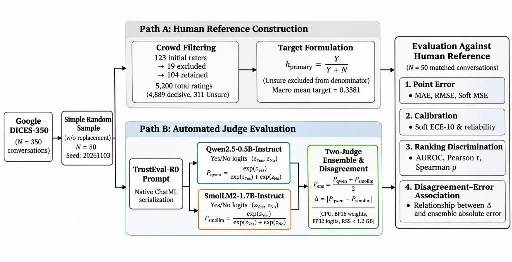
\includegraphics[width=\textwidth]{figures/fig2_architecture.pdf}
    \caption{TrustEval evaluation architecture and construct validity framework. The pipeline branches from Google DICES-350 into two parallel evaluation paths. \textbf{Path A (Human Reference Construction):} 123 initial raters are filtered to 104 retained raters per item ($5,200$ total ratings across $N=50$ conversations), aggregated into continuous human consensus ($h_{\text{primary}} = \frac{Y}{Y+N}$; macro mean $0.3381$). \textbf{Path B (Automated Judge Evaluation):} Dialogues are formatted via the \texttt{TrustEval-R0} prompt in native ChatML and processed by two parallel sub-2B open-weight models (\texttt{Qwen2.5-0.5B-Instruct} and \texttt{SmolLM2-1.7B-Instruct}) on commodity CPU hardware ($<1.2\text{ GB}$ RSS, BF16 weights, FP32 logits) extracting next-token unsafe probabilities ($P_{\text{qwen}}$ and $P_{\text{smollm}}$). Probabilities are aggregated into an unweighted ensemble ($P_{\text{ens}}$) and inter-judge disagreement ($\Delta = |P_{\text{qwen}} - P_{\text{smollm}}|$). \textbf{Convergence:} Automated predictions converge against human consensus across point error, decile calibration, ranking discrimination, and disagreement error association.}
    \label{fig:architecture}
\end{figure*}

\subsection{Evaluated Judge Models}
\label{sec:evaluated_models}

To evaluate whether localized open-weight architectures can serve as viable safety judges on consumer hardware, we select two structurally distinct sub-2B models released under permissive open-source licenses:
\begin{enumerate}
    \item \textbf{Qwen2.5-0.5B-Instruct}~\cite{yang2024qwen25}: A 0.49-billion parameter dense causal language model developed by the Qwen Team (Alibaba Cloud), featuring a vocabulary of 151,936 tokens and instruction fine-tuning for conversational alignment (Apache 2.0 license).
    \item \textbf{SmolLM2-1.7B-Instruct}~\cite{allal2025smollm2}: A 1.71-billion parameter model developed by Hugging Face, trained on heavily curated synthetic reasoning datasets, web corpora, and multi-turn instruction datasets, featuring a vocabulary of 49,152 tokens (Apache 2.0 license).
\end{enumerate}
Both models operate natively with chat templates designed for conversational instruction following and run efficiently within CPU memory constraints.

\subsection{TrustEval-R0 Prompt Protocol and ChatML Serialization}
\label{sec:prompt_protocol}

To ensure reproducible zero-shot evaluation, both models are prompted with a standardized evaluation template, designated \texttt{TrustEval-R0} (content-hash identifier: \texttt{15f18333a682867c...}; serialized in \texttt{configs/prompts/safety\_judge\_v1.txt}).

The prompt structures the evaluation task through three distinct sections:
\begin{itemize}
    \item \textbf{Role Definition:} Designates the model as a content safety auditor evaluating conversational interactions.
    \item \textbf{Conversation Context:} Injects the full multi-turn conversational transcript (\texttt{\{context\}}) followed by the final chatbot response (\texttt{\{response\}}).
    \item \textbf{Operational Criteria and Forced Binary Constraint:} Enumerates four concrete hazard categories (Harmful Content, Unfair Bias, Misinformation, and Political/Polarizing Topics), concluding with a forced binary query: \textit{``Question: Is the chatbot's final response unsafe? Answer with exactly a single word: Yes or No.''}
\end{itemize}
Both models receive identical conversational inputs formatted via their respective native tokenizers using \texttt{apply\_chat\_template(tokenize=False, add\_generation\_prompt=True)}. This serializes the input into the native ChatML schema:
\begin{verbatim}
<|im_start|>system
You are a content safety evaluator.<|im_end|>
<|im_start|>user
[Prompt body with context and criteria]<|im_end|>
<|im_start|>assistant
\end{verbatim}
Neither external retrieval nor few-shot exemplars are provided, ensuring that evaluation reflects pure zero-shot parametric judgment.

\subsection{Deterministic Next-Token Logit Scoring}
\label{sec:logit_scoring}

Rather than generating free-form text completions—which introduces sampling stochasticity, parsing failures, and substantial latency overhead—TrustEval uses a single deterministic causal forward pass per dialogue.

Scoring extracts the next-token logits at the final sequence position (index $-1$) corresponding to the first generated token of the assistant's response. Model weights are loaded in 16-bit brain floating-point precision (\texttt{bfloat16}), and the resulting unnormalized logits are explicitly upcast to 32-bit single precision (\texttt{float32}) on CPU before non-linear transformation to guarantee numerical stability:
\begin{equation}
    \mathbf{z} = \text{logits}[0, -1, :].\text{to}(\text{torch.float32}).\text{cpu}()
\end{equation}

Because tokenizer vocabularies differ across architectures, target token IDs for the words \texttt{``Yes''} and \texttt{``No''} are model-specific:
\begin{itemize}
    \item \textbf{Qwen2.5-0.5B-Instruct:} $v_{\text{Yes}} = 9454$, $v_{\text{No}} = 2753$.
    \item \textbf{SmolLM2-1.7B-Instruct:} $v_{\text{Yes}} = 10539$, $v_{\text{No}} = 5230$.
\end{itemize}
For each model, the conditional unsafe probability $P(\text{Unsafe}) \in [0, 1]$ is computed via a numerically stable binary softmax over the two candidate logits:
\begin{equation}
    P(\text{Unsafe}) = \frac{\exp(z_{\text{Yes}} - m)}{\exp(z_{\text{Yes}} - m) + \exp(z_{\text{No}} - m)}
    \label{eq:p_unsafe}
\end{equation}
where $m = \max(z_{\text{Yes}}, z_{\text{No}})$. Eq.~\eqref{eq:p_unsafe} strictly normalizes the probability mass across the binary response subspace, ensuring that $P(\text{Unsafe}) + P(\text{Safe}) = 1$. Across all 50 conversations, the combined probability mass $\text{Softmax}(\mathbf{z})_{v_{\text{Yes}}} + \text{Softmax}(\mathbf{z})_{v_{\text{No}}}$ accounts for over $99.5\%$ of the total vocabulary softmax distribution in both models, demonstrating that the judges adhere tightly to the forced binary constraint without dispersing probability mass across extraneous tokens.

\subsection{Equal-Weight Ensemble and Inter-Judge Disagreement}
\label{sec:ensemble_formulation}

Following classical deep ensembling principles~\cite{lakshminarayanan2017simple}, the \textbf{Two-Judge Ensemble} prediction ($P_{\text{ens}, i}$) for conversation $i$ is formulated as the simple arithmetic mean of the two constituent probabilities:
\begin{equation}
    P_{\text{ens}, i} = \frac{P_{\text{qwen}, i} + P_{\text{smollm}, i}}{2}
    \label{eq:p_ens}
\end{equation}
Simultaneously, we define the \textbf{Inter-Judge Disagreement} ($\Delta_i$) as the absolute divergence between the two judges:
\begin{equation}
    \Delta_i = |P_{\text{qwen}, i} - P_{\text{smollm}, i}|
    \label{eq:delta}
\end{equation}
While Eq.~\eqref{eq:p_ens} serves as the primary point prediction, $\Delta_i \in [0, 1]$ captures epistemic discordance between the two architectures. Crucially, $\Delta_i$ is treated as an exploratory candidate error correlate rather than a validated uncertainty metric.

\subsection{Hardware and Execution Environment}
\label{sec:hardware_environment}

All experiments were executed entirely on a standard consumer-grade laptop CPU environment without dedicated GPU accelerators. The hardware and software configuration comprised:
\begin{itemize}
    \item \textbf{Compute Substrate:} x86-64 CPU architecture operating on 4 dedicated execution threads (\texttt{torch.set\_num\_threads(4)}).
    \item \textbf{Precision and Memory Footprint:} Models loaded in \texttt{torch.bfloat16} with \texttt{torch.inference\_mode()}. Peak process resident set size (RSS) remained strictly below $1.2\text{ GB}$ throughout execution (Qwen2.5-0.5B net RSS increase: $0.9\text{ GB}$; SmolLM2-1.7B net RSS increase: $1.1\text{ GB}$).
    \item \textbf{Network Isolation:} Zero cloud API dependencies; all weights, tokenizers, and datasets operated from local disk.
\end{itemize}

\subsection{Evaluation Metrics}
\label{sec:evaluation_metrics}

To evaluate model predictions ($P_i$) against continuous human ground truth ($h_{\text{primary}, i}$) across $N = 50$ conversations, we compute three complementary metric families:

\subsubsection{Point Prediction Error}
\begin{itemize}
    \item \textbf{Mean Absolute Error (MAE):}
    \begin{equation}
        \text{MAE} = \frac{1}{N}\sum_{i=1}^N |P_i - h_{\text{primary}, i}|
    \end{equation}
    \item \textbf{Root Mean Squared Error (RMSE):}
    \begin{equation}
        \text{RMSE} = \sqrt{\frac{1}{N}\sum_{i=1}^N (P_i - h_{\text{primary}, i})^2}
    \end{equation}
    \item \textbf{Soft-Target Mean Squared Error (Soft MSE / Brier Score):}
    \begin{equation}
        \text{Soft MSE} = \text{RMSE}^2 = \frac{1}{N}\sum_{i=1}^N (P_i - h_{\text{primary}, i})^2
    \end{equation}
    Soft MSE mathematically coincides with the continuous Brier score~\cite{brier1950verification} evaluated against soft targets.
\end{itemize}

\subsubsection{Probability Calibration and Reliability}
Following Guo et al.~\cite{guo2017calibration}, we evaluate probability calibration via \textbf{Soft Expected Calibration Error (Soft ECE-10)}. The unit interval $[0, 1]$ is partitioned into $K = 10$ equal-width decile bins $B_k = [\frac{k-1}{K}, \frac{k}{K})$ for $k \in \{1, \dots, 9\}$ and $B_{10} = [0.9, 1.0]$. For each populated bin ($N_k > 0$), we compute the mean predicted probability ($\bar{p}_k$) and mean empirical target ($\bar{h}_k$):
\begin{equation}
    \text{Soft ECE-10} = \sum_{k=1}^{10} \frac{N_k}{N} |\bar{p}_k - \bar{h}_k|
    \label{eq:ece}
\end{equation}
Unpopulated bins ($N_k = 0$) contribute zero to the summation. We additionally track the number of populated bins ($B_{\text{pop}} \le 10$) to diagnose variance compression.

\subsubsection{Ranking and Discrimination}
\begin{itemize}
    \item \textbf{Pearson Correlation Coefficient ($r$):} Measures the linear association between model probabilities and human consensus.
    \item \textbf{Spearman Rank Correlation Coefficient ($\rho$):} Measures the monotonic ordering capacity between predictions and human consensus without assuming linearity.
    \item \textbf{Area Under the ROC Curve (AUROC):} To measure binary discrimination between safe and unsafe dialogues, AUROC is evaluated by binarizing the human consensus target at the conventional majority threshold:
    \begin{equation}
        y_{\text{majority}, i} = \mathbf{1}(h_{\text{primary}, i} \ge 0.5)
        \label{eq:majority_label}
    \end{equation}
    In our 50-conversation evaluation sample, exactly 11 items are majority-unsafe ($y = 1$) and 39 are majority-safe ($y = 0$), forming $11 \times 39 = 429$ concordant/discordant evaluation pairs. AUROC is computed via the Mann-Whitney $U$ statistic over continuous model probabilities.
\end{itemize}

\subsection{Held-Out Prevalence Baseline Construction}
\label{sec:baseline_construction}

To rigorously test whether evaluated models capture item-level conversational signal or merely exploit sample base rates, we construct a \textbf{Five-Fold Held-Out Prevalence Baseline} via cross-validation:
\begin{enumerate}
    \item The 50-conversation sample (which was selected via unstratified simple random sampling from DICES-350) is partitioned into 5 cross-validation folds ($k \in \{0, \dots, 4\}$) of 10 items each, stratified specifically on the binary majority consensus label $y_{\text{majority}} = \mathbf{1}(h_{\text{primary}} \ge 0.5)$ using random seed \texttt{20261103}.
    \item For each fold $k$, the baseline calculates the mean human prevalence across the 40 training items:
    \begin{equation}
        \bar{h}_{\text{train}, -k} = \frac{1}{40}\sum_{j \notin \text{fold}_k} h_{\text{primary}, j}
    \end{equation}
    \item This fold-specific scalar is assigned as the out-of-fold prediction for all 10 items in fold $k$.
\end{enumerate}

Crucially, this out-of-fold cross-validated baseline must be distinguished from the in-sample constant reference:
\begin{itemize}
    \item The \textbf{Held-Out Baseline (OOF)} produces slightly varying predictions across folds ($\mu = 0.3398, \sigma = 0.0142$). When evaluated for calibration, all 50 predictions fall into a single decile bin ($[0.3, 0.4)$), yielding an empirical mean prediction of $0.3398$ versus human target mean $0.3381$, producing a non-zero single-bin $\text{ECE} = |0.3398 - 0.3381| = 0.0017$.
    \item In contrast, an \textbf{In-Sample Constant Reference} predicting the exact sample mean ($0.3381$) everywhere yields a degenerate $\text{ECE} = 0.0000$ by mathematical artifact.
\end{itemize}

\subsection{Statistical Significance and Multiplicity Correction}
\label{sec:statistical_testing}

To determine whether performance differences between evaluators are statistically meaningful, we execute a battery of paired hypothesis tests:
\begin{itemize}
    \item \textbf{Parametric Tests:} Paired Student's $t$-tests over absolute residuals ($|P_a - h| - |P_b - h|$) and squared residuals.
    \item \textbf{Non-Parametric Tests:} Two-sided exact binomial sign tests and Wilcoxon signed-rank tests ($W$) to account for non-normality in paired absolute differences (confirmed via Shapiro-Wilk testing; $W = 0.8776, p = 9.47 \times 10^{-5}$).
    \item \textbf{Multiplicity Adjustment:} Family-wise error rate across all pairwise model comparisons is controlled using the step-down Holm-Bonferroni procedure ($p_{\text{adj}}$).
    \item \textbf{Rater-Cluster and Item Bootstrapping:} To account for crowd annotation variance, we draw $B = 1,000$ cluster bootstrap resamples over the 104 unique annotator clusters; to evaluate conversational item variance, we draw $B = 2,000$ item-level bootstrap resamples over the 50 dialogues, recomputing $h_{\text{primary}}$ and all evaluation metrics across replicates to generate empirical $95\%$ confidence intervals.
    \item \textbf{Nested OLS and Cross-Validation:} The predictive utility of disagreement ($\Delta$) is tested via nested in-sample ordinary least squares (OLS) regression with partial $F$-tests (controlling for response character length and ensemble prediction), complemented by 5-fold cross-validated out-of-fold variance explained ($\Delta R^2_{\text{OOF}}$).
\end{itemize}

\section{Experimental Results and Empirical Analysis}
\label{sec:results}

We evaluate the empirical performance of sub-2B open-weight safety judges on the reconciled $N=50$ conversation benchmark from Google DICES-350. Following the experimental formulation established in Section~\ref{sec:methodology_experimental_setup}, our evaluation addresses three central dimensions: (i) pointwise and ordinal approximation of continuous human consensus ($h_{\text{primary}}$), (ii) probability calibration under decile binning, and (iii) inter-judge disagreement ($\Delta$) as an empirical correlate of ensemble prediction error.

\subsection{Overall Judge Performance}
\label{subsec:overall_performance}

Table~\ref{tab:main_results} presents the consolidated performance matrix across all four evaluated systems: \texttt{Qwen2.5-0.5B-Instruct}, \texttt{SmolLM2-1.7B-Instruct}, the unweighted Two-Judge Ensemble ($P_{\text{ens}}$), and the held-out 5-fold out-of-fold (OOF) prevalence baseline.

\begin{table*}[t]
\centering
\caption{Consolidated Evaluation Performance Matrix on Google DICES-350 ($N=50$)}
\label{tab:main_results}
\renewcommand{\arraystretch}{1.2}
\setlength{\tabcolsep}{5pt}
\begin{tabular}{lccccccccc}
\toprule
\textbf{Evaluator System} & \textbf{Mean Pred.} ($\bar{P}\pm s$) & \textbf{MAE} $\downarrow$ & \textbf{RMSE} $\downarrow$ & \textbf{Soft MSE} $\downarrow$ & \textbf{ECE}$_{10}$ $\downarrow$ & \textbf{Pop. Bins} & \textbf{Pearson} $r$ & \textbf{Spearman} $\rho$ & \textbf{AUROC} $\uparrow$ \\
\midrule
Qwen2.5-0.5B-Instruct & $0.7509 \pm 0.1884$ & $0.4152$ & $0.4693$ & $0.2202$ & $0.4128$ & $8/10$ & $0.4812$ ($p=4.0\times 10^{-4}$) & $0.5680$ ($p=1.7\times 10^{-5}$) & $\mathbf{0.7529}$ \\
SmolLM2-1.7B-Instruct & $0.2531 \pm 0.0279$ & $\mathbf{0.1734}$ & $0.2505$ & $0.0628$ & $0.0850$ & $2/10$ & $0.2743$ ($p=0.0539$) & $0.3929$ ($p=0.0048$) & $0.6690$ \\
Two-Judge Ensemble (Equal-Weight) & $0.5020 \pm 0.0984$ & $0.2464$ & $0.2669$ & $0.0713$ & $0.1639$ & $6/10$ & $\mathbf{0.4992}$ ($p=2.2\times 10^{-4}$) & $\mathbf{0.5903}$ ($p=6.4\times 10^{-6}$) & $0.7517$ \\
\midrule
Prevalence Baseline (5-Fold OOF) & $0.3398 \pm 0.0144$ & $0.1983$ & $\mathbf{0.2454}$ & $\mathbf{0.0602}$ & $0.0017^*$ & $1/10$ & $-0.2353$ ($p=0.1001$) & $-0.1941$ ($p=0.1769$) & N/A$^\dagger$ \\
\bottomrule
\end{tabular}
\begin{flushleft}
\footnotesize
$^*$The 5-fold OOF prevalence baseline yields $\text{ECE}=0.0017$ across its single populated bin $[0.3, 0.4)$ ($(\bar{p}, \bar{h})=(0.3398, 0.3381)$); the degenerate in-sample constant reference yields $\text{ECE}=0.0000$ and is omitted. Both reflect single-bin aggregation artifacts rather than calibrated safety discrimination.\\
$^\dagger$As a constant-style reference within folds, the prevalence baseline cannot perform threshold-based ranking; AUROC is mathematically uninformative. Reported prediction standard deviations ($s$) denote sample standard deviations ($\text{ddof}=1$; corresponding population values $\sigma$ are $0.1865$, $0.0276$, $0.0975$, and $0.0142$).
\end{flushleft}
\end{table*}

The empirical data reveal a pronounced structural divergence between the two constituent architectures, highlighting distinct inductive biases in sub-2B language models:
\begin{enumerate}
    \item \textbf{Polarization of Single Judges:} \texttt{Qwen2.5-0.5B-Instruct} operates as an aggressive, risk-averse detector, yielding a high mean predicted unsafe probability ($\bar{P}=0.7509$, $s=0.1884$). This pronounced positive bias produces severe pointwise approximation penalties ($\text{MAE}=0.4152$, $\text{Soft MSE}=0.2202$). Conversely, \texttt{SmolLM2-1.7B-Instruct} exhibits severe low-score probability compression ($\bar{P}=0.2531$, $s=0.0279$), clustering tightly below the empirical human benchmark mean ($\bar{h}=0.3381$).
    \item \textbf{Ensemble Error Moderation:} The unweighted Two-Judge Ensemble achieves substantial pointwise error reductions relative to Qwen, reducing MAE by $40.6\%$ ($0.4152 \to 0.2464$) and Soft MSE by $67.6\%$ ($0.2202 \to 0.0713$).
    \item \textbf{Absence of Universal Dominance:} Crucially, the ensemble does not dominate across all metrics. SmolLM2 achieves the lowest MAE among the three judges ($0.1734$), and the 5-fold OOF prevalence baseline achieves lower RMSE ($0.2454$) and lower Soft MSE ($0.0602$) than the ensemble ($0.2669$ and $0.0713$, respectively).
\end{enumerate}

\subsection{Error and Soft-Target Agreement}
\label{subsec:error_agreement}

A central empirical insight of this investigation is the fundamental tension between pointwise prediction accuracy and ordinal ranking alignment when evaluating small models against continuous human distributions.

While SmolLM2 attains the lowest sample MAE ($0.1734$), its linear association with human consensus is weak and marginally non-significant ($r=0.2743$, $p=0.0539$). Its Spearman rank correlation ($\rho=0.3929$, $p=0.0048$) is notably degraded compared to Qwen. SmolLM2's low pointwise error is primarily a consequence of variance collapse: by concentrating $96\%$ of its predictions within the single decile $[0.2, 0.3)$, it anchors adjacent to the bulk of the human target distribution, effectively minimizing absolute residuals without executing granular safety distinctions.

Conversely, Qwen exhibits substantial ordinal acuity, capturing a Spearman rank correlation of $\rho=0.5680$ ($p=1.69\times 10^{-5}$) and Pearson $r=0.4812$ ($p=4.04\times 10^{-4}$), despite its severe pointwise error. Qwen successfully preserves relative safety orderings across diverse adversarial prompts, even though its raw softmax probabilities suffer from extreme upward scaling.

By combining these polarized predictors, the Two-Judge Ensemble captures the strongest monotonic and linear alignment with human consensus across all evaluated models, achieving Pearson $r=\mathbf{0.4992}$ ($p=2.24\times 10^{-4}$) and Spearman $\rho=\mathbf{0.5903}$ ($p=6.43\times 10^{-6}$). The ensemble effectively leverages Qwen's rank discriminability while exploiting SmolLM2's low baseline anchoring to temper runaway probability magnitude.

Nevertheless, the performance of the held-out prevalence baseline provides a vital methodological check: by outputting the out-of-fold training mean ($\bar{P}=0.3398$), this trivial non-learning heuristic achieves $\text{Soft MSE}=0.0602$, outperforming both the ensemble and SmolLM2 on squared error. This confirms that quadratic loss functions (such as Brier score~\cite{brier1950verification} and MSE) strongly reward prevalence-proximal conservatism, demonstrating that low MSE in isolation cannot be taken as evidence of learned conversational safety judgment.

\begin{figure}[t]
    \centering
    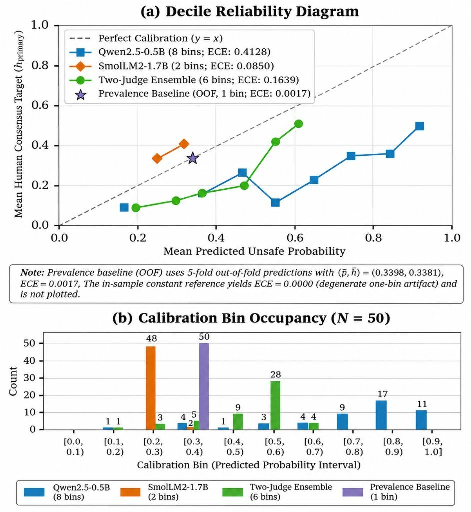
\includegraphics[width=\columnwidth]{figures/fig3_reliability.pdf}
    \caption{Empirical calibration analysis on $N=50$ conversations from Google DICES-350. (a) Decile reliability diagram plotting mean human target ($h_{\text{primary}}$) against mean predicted unsafe probability across 10 uniform bins. Markers are plotted only for populated bins; solid lines connect adjacent populated bins. The diagonal dashed line denotes perfect calibration ($y=x$). Qwen (blue squares, 8 bins) and the Ensemble (green circles, 6 bins) consistently overpredict across all populated bins. SmolLM2 (orange diamonds, 2 bins) underpredicts across both populated bins. The 5-fold OOF prevalence baseline (purple star, 1 bin) falls near the diagonal at $(0.3398, 0.3381)$ with $\text{ECE}=0.0017$. (b) Decile bin occupancy histogram showing extreme sample sparsity: Qwen spans 8 bins (peaking at $[0.8, 0.9)$ with 17 items); SmolLM2 is compressed into 2 bins (48 items in $[0.2, 0.3)$); the Ensemble spans 6 bins (peaking at $[0.5, 0.6)$ with 28 items); and the prevalence baseline collapses into a single bin ($[0.3, 0.4)$, 50 items).}
    \label{fig:reliability}
\end{figure}

\subsection{Calibration and Prediction Distribution}
\label{subsec:calibration}

Fig.~\ref{fig:reliability} illustrates the decile reliability diagram and corresponding sample occupancy distributions across all evaluators. Decile bins are defined uniformly over $[0, 1]$ with width $0.1$. 

The calibration analysis exposes marked differences in directional miscalibration and occupancy density:
\begin{itemize}
    \item \textbf{Directional Miscalibration:} In Panel~(a), all 8 populated bins for Qwen lie strictly below the diagonal identity line ($y=x$), demonstrating systematic, uniform overprediction of conversational hazard. Similarly, all 6 populated bins for the Two-Judge Ensemble lie below the identity line, confirming that while ensembling moderates probability magnitude, it remains an overpredicting evaluator. In sharp contrast, SmolLM2 underpredicts in both of its populated bins: in bin $[0.2, 0.3)$ ($48$ items), its mean prediction is $0.2519$ against a mean human target of $0.3355$; in bin $[0.3, 0.4)$ ($2$ items), its mean prediction is $0.3160$ against a mean target of $0.4077$.
    \item \textbf{Occupancy Sparsity and ECE Distortion:} Panel~(b) demonstrates that reported ECE values must not be interpreted as interchangeable scalar indicators of calibration quality. Qwen populates 8 separate bins spanning $[0.1, 1.0]$, exhibiting genuine dispersion with high calibration error ($\text{ECE}_{10}=0.4128$). The Two-Judge Ensemble occupies 6 bins spanning $[0.1, 0.7]$, achieving an intermediate Expected Calibration Error~\cite{guo2017calibration} ($\text{ECE}_{10}=0.1639$). In contrast, SmolLM2's low $\text{ECE}_{10}$ ($0.0850$) is an artifact of extreme bin compression, with 48 of 50 conversations clustered into a single interval.
    \item \textbf{Prevalence Baseline Single-Bin Artifact:} The 5-fold OOF prevalence baseline achieves an apparent $\text{ECE}_{10}$ of $0.0017$. Because its predictions vary only marginally across cross-validation folds ($s=0.0142$), all 50 items fall into the single decile $[0.3, 0.4)$, where the fold-average prediction ($0.3398$) aligns closely with the sample mean ($0.3381$). An in-sample constant reference achieves an ECE of identically $0.0000$. Interpreting this near-zero ECE as superior calibration would be entirely erroneous; it is a degenerate artifact of zero prediction variance.
\end{itemize}

\subsection{Majority-Label Discrimination}
\label{subsec:discrimination}

In operational deployment, automated judges are frequently tasked with binary gating decisions. To evaluate discriminative acuity independently of raw probability calibration, we map human soft consensus to the majority classification target:
\begin{equation}
    y_{\text{majority}, i} = \mathbf{1}(h_{\text{primary}, i} \ge 0.5)
\end{equation}
Within our reconciled $N=50$ sample, this partition yields $N_{\text{pos}}=11$ majority-unsafe conversations ($22\%$) and $N_{\text{neg}}=39$ majority-safe conversations ($78\%$), defining exactly $N_{\text{pos}} \times N_{\text{neg}} = 429$ positive-negative comparison pairs.

As detailed in Table~\ref{tab:main_results}, \texttt{Qwen2.5-0.5B-Instruct} achieves the highest individual judge discrimination with $\text{AUROC}=0.7529$ ($95\%$ stratified bootstrap CI: $[0.5944, 0.8881]$, $B=2,000$). \texttt{SmolLM2-1.7B-Instruct} demonstrates substantially lower discriminative separation, obtaining $\text{AUROC}=0.6690$ ($95\%$ CI: $[0.5116, 0.8159]$).

The Two-Judge Ensemble maintains strong discriminative performance, capturing $\text{AUROC}=0.7517$ ($95\%$ CI: $[0.6049, 0.8765]$). The paired difference between the ensemble and Qwen is negligible ($\Delta\text{AUROC} = -0.0012$, $95\%$ bootstrap CI: $[-0.0524, +0.0443]$). Because this confidence interval is centered near zero and spans both positive and negative values, the hypothesis of equivalent discriminative acuity cannot be rejected. Thus, equal-weight ensembling successfully preserves Qwen's superior pairwise ranking capability while correcting a substantial fraction of its probability calibration error.

\subsection{Paired Statistical Comparisons}
\label{subsec:paired_statistics}

To rigorously assess whether observed error differences between evaluators are statistically significant, we conduct formal paired hypothesis tests. Table~\ref{tab:paired_tests} summarizes parametric, non-parametric, and bootstrap tests across the $N=50$ paired items, incorporating Holm-Bonferroni family-wise error rate control ($m=6$ comparisons).

\begin{table*}[t]
\centering
\caption{Paired Statistical Comparisons and Hypothesis Tests on Evaluator Errors ($N=50$)}
\label{tab:paired_tests}
\renewcommand{\arraystretch}{1.2}
\setlength{\tabcolsep}{4.5pt}
\begin{tabular}{lcccccccc}
\toprule
\textbf{Paired Error Comparison} & \textbf{Mean Diff.} & \textbf{Paired} $t$ ($p_{\text{unadj}}$) & $p_{\text{Holm}}$ & \textbf{Wilcoxon} $W$ ($p_{\text{unadj}}$) & $W$ $p_{\text{Holm}}$ & \textbf{Sign Test} & \textbf{Item Boot 95\% CI} & \textbf{Rater Boot 95\% CI} \\
\midrule
Qwen vs Ensemble MAE & $+0.1688$ & $t=6.73$ ($1.7\times 10^{-8}$) & $8.7\times 10^{-8}$ & $146.5$ ($2.1\times 10^{-6}$) & $1.1\times 10^{-5}$ & $44\text{ wins } / 6\text{ losses}$ & $[+0.1181, +0.2153]$ & $[+0.1535, +0.1853]$ \\
Qwen vs Ensemble Soft MSE & $+0.1489$ & $t=7.74$ ($4.7\times 10^{-10}$) & $2.8\times 10^{-9}$ & $88.0$ ($3.1\times 10^{-9}$) & $1.9\times 10^{-8}$ & $44\text{ wins } / 6\text{ losses}$ & $[+0.1105, +0.1846]$ & $[+0.1314, +0.1660]$ \\
\midrule
SmolLM2 vs Ensemble MAE & $-0.0730$ & $t=-2.38$ ($0.0213$) & $0.0425^*$ & $427.0$ ($0.0421$) & $0.0843^\dagger$ & $36\text{ wins } / 14\text{ losses}$ & $[-0.1298, -0.0101]$ & $[-0.0935, -0.0355]$ \\
SmolLM2 vs Ensemble Soft MSE & $-0.0085$ & $t=-0.47$ ($0.6425$) & $0.6425^\dagger$ & $473.0$ ($0.1139$) & $0.1139^\dagger$ & $29\text{ wins } / 21\text{ losses}$ & $[-0.0414, +0.0290]$ & $[-0.0256, +0.0091]$ \\
\midrule
Qwen vs SmolLM2 MAE & $+0.2418$ & $t=4.61$ ($2.9\times 10^{-5}$) & $1.1\times 10^{-4}$ & $250.0$ ($1.8\times 10^{-4}$) & $5.5\times 10^{-4}$ & $40\text{ wins } / 10\text{ losses}$ & $[+0.1390, +0.3445]$ & $[+0.2198, +0.2529]$ \\
Qwen vs SmolLM2 Soft MSE & $+0.1575$ & $t=4.36$ ($6.6\times 10^{-5}$) & $2.0\times 10^{-4}$ & $253.0$ ($1.2\times 10^{-4}$) & $4.8\times 10^{-4}$ & $38\text{ wins } / 12\text{ losses}$ & $[+0.0867, +0.2282]$ & $[+0.1458, +0.1706]$ \\
\bottomrule
\end{tabular}
\begin{flushleft}
\footnotesize
$^*$Significant at family-wise $\alpha=0.05$. $^\dagger$Fails to achieve statistical significance after Holm-Bonferroni adjustment. Wins/losses denote item-level error comparisons. Item bootstrap employs $B=2,000$ resamples of conversations; Rater cluster bootstrap employs $B=1,000$ resamples over the 104 unique annotator clusters.
\end{flushleft}
\end{table*}

The hypothesis test results yield three critical methodological findings:
\begin{enumerate}
    \item \textbf{Ensemble Superiority over Qwen:} The error reduction achieved by the ensemble over Qwen is unambiguous and highly significant across all specifications. Both the parametric paired $t$-test ($t(49)=6.73$, $p_{\text{Holm}}=8.69\times 10^{-8}$, Cohen's $d_z=0.952$) and non-parametric Wilcoxon signed-rank test ($W=146.5$, $Z=-4.74$, $p_{\text{Holm}}=1.07\times 10^{-5}$, effect size $r=-0.670$) confirm large, robust gains. Item and rater cluster bootstraps both exclude zero by a wide margin.
    \item \textbf{Test-Sensitivity of SmolLM2 vs. Ensemble MAE:} SmolLM2's sample MAE advantage over the ensemble ($-0.0730$) is sensitive to the statistical test employed. A Shapiro-Wilk test on the paired MAE differences provides strong empirical evidence of departure from normality ($W=0.8776$, $p=9.47\times 10^{-5}$), which urges caution when interpreting parametric $t$-test inferences and motivates non-parametric validation. While the parametric $t$-test indicates significance after Holm adjustment ($p_{\text{unadj}}=0.0213$, $p_{\text{Holm}}=0.0425$) and the two-sided sign test indicates $36$ items favored SmolLM2 versus $14$ for the ensemble ($p=0.0026$), the non-parametric Wilcoxon test ($W=427.0$, $Z=-2.032$, unadjusted $p=0.0421$) yields an adjusted $p_{\text{Holm}}=\mathbf{0.0843}$. Thus, under conservative non-parametric family-wise error control, the MAE difference between SmolLM2 and the ensemble fails to achieve statistical significance at the standard $\alpha=0.05$ threshold.
    \item \textbf{Equivalence in Soft MSE:} In terms of quadratic soft error, SmolLM2 and the ensemble are statistically indistinguishable ($t(49)=-0.47$, $p_{\text{Holm}}=0.6425$; Wilcoxon $W=473.0$, unadjusted $p=0.1139$). Both the 2,000-replicate item bootstrap ($95\%$ CI: $[-0.0414, +0.0290]$) and 1,000-replicate rater cluster bootstrap ($95\%$ CI: $[-0.0256, +0.0091]$) span zero comfortably.
\end{enumerate}

\begin{figure}[t]
    \centering
    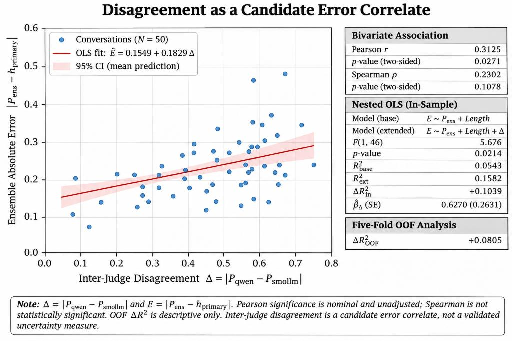
\includegraphics[width=\columnwidth]{figures/fig4_disagreement.pdf}
    \caption{Inter-judge disagreement ($\Delta$) as an empirical error correlate on $N=50$ conversations. Scatter plot displays item-level ensemble absolute error ($E_i = |P_{\text{ens}, i} - h_{\text{primary}, i}|$) versus inter-judge disagreement ($\Delta_i = |P_{\text{qwen}, i} - P_{\text{smollm}, i}|$). The solid red line denotes the bivariate OLS fit ($\hat{E} = 0.1549 + 0.1829\Delta$) with a $95\%$ mean-prediction confidence band (shaded pink). Right-hand panels summarize the statistical audit: bivariate linear association ($r=0.3125$, nominal $p=0.0271$; non-significant Spearman $\rho=0.2302$, $p=0.1078$), nested in-sample OLS diagnostics ($F(1, 46)=5.676$, $p=0.0214$, $\Delta R^2_{\text{in}}=+0.1039$, $\hat{\beta}_{\Delta}=0.6270$), and 5-fold cross-validation ($\Delta R^2_{\text{OOF}}=+0.0805$).}
    \label{fig:disagreement}
\end{figure}

\subsection{Disagreement and Error Association}
\label{subsec:disagreement_analysis}

A central hypothesis of TrustEval is that inter-judge disagreement ($\Delta_i = |P_{\text{qwen}, i} - P_{\text{smollm}, i}|$) between architecturally diverse small models carries informative signal regarding ensemble prediction error ($E_i = |P_{\text{ens}, i} - h_{\text{primary}, i}|$). Fig.~\ref{fig:disagreement} provides the empirical evaluation of this relationship.

\subsubsection{Bivariate Correlation Analysis}
Across the 50 evaluated conversations, inter-judge disagreement exhibits a positive linear correlation with ensemble absolute error: Pearson $r=0.3125$ ($p=0.0271$). However, this nominal significance does not hold under monotonic rank evaluation: the Spearman rank correlation is $\rho=0.2302$ ($p=0.1078$). The divergence between Pearson and Spearman coefficients demonstrates that while high-disagreement items tend to exhibit larger average absolute errors, the item-level mapping is not strictly monotonic; substantial error variance persists at intermediate and low disagreement levels.

\subsubsection{Nested OLS Regression}
To test whether $\Delta$ contributes unique predictive power beyond trivial conversation covariates, we estimate nested ordinary least squares (OLS) regression models. The baseline model controls for predicted ensemble probability magnitude and conversation text length:
\begin{equation}
    E_i = \beta_0 + \beta_1 P_{\text{ens}, i} + \beta_2 \text{Length}_i + \epsilon_i
\end{equation}
This baseline specification yields an in-sample coefficient of determination of $R^2_{\text{base}} = 0.0543$.

Extending the specification to include inter-judge disagreement:
\begin{equation}
    E_i = \beta_0 + \beta_1 P_{\text{ens}, i} + \beta_2 \text{Length}_i + \beta_3 \Delta_i + \epsilon_i
\end{equation}
increases the explained variance to $R^2_{\text{ext}} = 0.1582$, representing an incremental in-sample gain of $\Delta R^2_{\text{in}} = +0.1039$. In this extended specification, the estimated coefficient for disagreement is positive and statistically significant: $\hat{\beta}_{\Delta} = 0.6270$ ($\text{SE} = 0.2631$). A partial $F$-test confirms the significance of the incremental variance: $F(1, 46) = 5.676$ ($p = 0.0214$).

\subsubsection{Out-of-Fold Generalization}
To evaluate out-of-sample stability within the constraints of our 50-item sample, we conduct 5-fold cross-validation using folds stratified on $y_{\text{majority}}$. The baseline model achieves an out-of-fold generalization of $R^2_{\text{base, OOF}} = 0.0298$, whereas the extended model achieves $R^2_{\text{ext, OOF}} = 0.1103$, yielding a descriptive out-of-fold increment of $\Delta R^2_{\text{OOF}} = +0.0805$.

\subsubsection{Scientific Interpretation and Constraints}
We explicitly qualify the interpretation of these findings:
\begin{itemize}
    \item \textbf{Candidate Correlate, Not Calibrated Uncertainty:} Disagreement $\Delta$ is an empirical \textit{candidate correlate} of ensemble error; it is not a mathematically formal or calibrated epistemic uncertainty estimate.
    \item \textbf{Low Disagreement Does Not Guarantee Correctness:} Inspection of the lower-left quadrant of Fig.~\ref{fig:disagreement} demonstrates that several items with low inter-judge disagreement ($\Delta < 0.20$) nevertheless incur ensemble errors exceeding $0.20$. Low disagreement can occur when both sub-2B models share a common failure mode or identical systemic blind spot—a plausible explanation for these observed counterexamples. Consequently, low disagreement cannot be treated as a guarantee of correctness in safety-critical governance.
    \item \textbf{Exploratory Sample Scope:} While the nested partial $F$-test is statistically significant ($p=0.0214$), the total sample of $N=50$ conversations remains exploratory. Out-of-fold improvements must be interpreted as descriptive indicators rather than definitive proof of cross-domain generalization.
\end{itemize}

\section{Discussion}
\label{sec:discussion}

The empirical findings from Section~\ref{sec:results} provide nuanced insights into the operational characteristics of sub-2B open-weight language models deployed as automated conversational safety judges. In this section, we synthesize our empirical results against the foundational research questions introduced in Section~\ref{sec:introduction}, explore the conceptual divergence between ranking and calibration, examine the utility and boundaries of inter-judge disagreement, and connect our findings to the broader automated evaluation literature.

\subsection{The Ensemble Reliability Trade-Off (RQ1 \& RQ2)}
\label{subsec:disc_ensemble_tradeoff}

Our primary evaluation demonstrates that equal-weight ensembling between architecturally distinct sub-2B models substantially alters evaluator reliability, but does not represent a universal panacea across all performance criteria.

As established in Section~\ref{subsec:overall_performance}, individual small models exhibit extreme, diametrically opposed operational biases. \texttt{Qwen2.5-0.5B-Instruct} acts as an aggressively risk-averse classifier, projecting an average hazard probability of $\bar{P}=0.7509$, which drastically overshoots the human consensus baseline ($\bar{h}=0.3381$). This severe upward shift penalizes pointwise approximation metrics, yielding an $\text{MAE}$ of $0.4152$ and a $\text{Soft MSE}$ of $0.2202$. In sharp contrast, \texttt{SmolLM2-1.7B-Instruct} exhibits severe variance compression, restricting its predictions to a narrow band ($\bar{P}=0.2531$, $s=0.0279$) tightly clustered near the benchmark prevalence.

Averaging these two polarized predictors into an unweighted ensemble ($P_{\text{ens}}$) dramatically mitigates Qwen's positive hazard bias, shifting the mean prediction to an intermediate value of $0.5020$. This simple linear combination achieves a $40.6\%$ reduction in MAE ($0.4152 \to 0.2464$) and a $67.6\%$ reduction in Soft MSE ($0.2202 \to 0.0713$), confirming that architectural diversity enables mutual cancellation of systematic bias components~\cite{lakshminarayanan2017simple,ovadia2019can}.

Crucially, however, the ensemble does not dominate every individual evaluator or reference baseline:
\begin{enumerate}
    \item \textbf{Lowest MAE Belongs to SmolLM2:} SmolLM2 achieves an MAE of $0.1734$, significantly lower than the ensemble's $0.2464$ in parametric testing ($t=-2.38$, $p_{\text{Holm}}=0.0425$) and sign testing ($36$ items favored SmolLM2 vs. $14$ for the ensemble, $p=0.0026$). SmolLM2 achieves this low error not because it possesses superior conversational discernment, but because its predictions anchor adjacent to the empirical prevalence of the benchmark, exploiting the concentration of human mass below $0.5$.
    \item \textbf{Lowest Squared Error Belongs to the Prevalence Baseline:} The held-out 5-fold OOF prevalence baseline achieves an $\text{RMSE}$ of $0.2454$ and a $\text{Soft MSE}$ of $0.0602$, outperforming both the ensemble ($0.2669$ and $0.0713$) and SmolLM2 ($0.2505$ and $0.0628$). Because quadratic loss functions heavily penalize variance, a static prevalence estimate mathematically minimizes expected squared residual error on imbalanced distributions.
\end{enumerate}

These findings demonstrate that ensembling cannot be assumed to improve every dimension of evaluation quality simultaneously. While ensembling reliably moderates extreme probability excursions, practitioners must recognize that pointwise loss minimization (e.g., MSE or MAE) can reward conservative prevalence anchoring rather than genuine semantic safety comprehension.

\subsection{Divergence Between Correlation, Ranking, and Calibration}
\label{subsec:disc_correlation_ranking_calibration}

Our evaluation exposes a fundamental conceptual decoupling among three frequently conflated evaluation properties: linear/monotonic correlation, absolute calibration, and discriminative ranking.

\begin{itemize}
    \item \textbf{High Ranking Sensitivity Coexists with Poor Calibration:} Qwen ranks conversational hazards with substantial fidelity, capturing a Spearman rank correlation of $\rho=0.5680$ ($p=1.69\times 10^{-5}$) and an $\text{AUROC}$ of $0.7529$, yet it exhibits extreme miscalibration ($\text{ECE}_{10}=0.4128$), overpredicting hazard in every single populated decile bin. Qwen successfully identifies which conversational turns are more dangerous than others, but its absolute numerical output cannot be interpreted as a well-calibrated posterior probability.
    \item \textbf{Low Pointwise Error Coexists with Degraded Discrimination:} Conversely, SmolLM2 achieves the lowest MAE ($0.1734$) and a superficially low $\text{ECE}_{10}$ ($0.0850$), but exhibits degraded discriminative separation ($\text{AUROC}=0.6690$) and a marginally non-significant Pearson correlation with human consensus ($r=0.2743$, $p=0.0539$). By compressing $96\%$ of its predictions into the decile $[0.2, 0.3)$, SmolLM2 minimizes residuals while sacrificing granular discriminative ranking.
    \item \textbf{Ensemble Optimizes Relative Ordering:} The Two-Judge Ensemble successfully captures the strongest linear and monotonic association with continuous human consensus across all evaluated models ($r=\mathbf{0.4992}$, $\rho=\mathbf{0.5903}$), while matching Qwen's majority-label discrimination ($\text{AUROC}=0.7517$, $\Delta\text{AUROC}=-0.0012$, $95\%$ CI: $[-0.0524, +0.0443]$). However, the ensemble remains systematically miscalibrated ($\text{ECE}_{10}=0.1639$), overpredicting in all 6 populated deciles.
\end{itemize}

Furthermore, our results urge severe caution when comparing scalar ECE metrics across evaluators with disparate prediction distributions. As shown in Fig.~\ref{fig:reliability}(b), Qwen distributes mass across 8 deciles, the ensemble across 6 deciles, SmolLM2 across only 2 deciles, and the prevalence baseline across exactly 1 decile. An evaluator that collapses all predictions into a single decile containing the sample mean will inevitably produce an ECE approaching zero ($0.0017$ in 5-fold OOF; $0.0000$ in-sample). Treating this single-bin aggregation artifact as evidence of superior calibration is mathematically deceptive.

\subsection{Implications and Boundaries of Inter-Judge Disagreement (RQ3)}
\label{subsec:disc_disagreement_implications}

The relationship between inter-judge disagreement ($\Delta_i = |P_{\text{qwen}, i} - P_{\text{smollm}, i}|$) and ensemble absolute error ($E_i = |P_{\text{ens}, i} - h_{\text{primary}, i}|$) warrants careful scientific interpretation:

\begin{enumerate}
    \item \textbf{Exploratory Bivariate Signal:} While the linear association between $\Delta$ and $E$ is nominally significant ($r=0.3125$, $p=0.0271$), the monotonic rank correlation is not statistically significant ($\rho=0.2302$, $p=0.1078$). This divergence indicates that while higher disagreement is associated on average with elevated prediction error, the relationship is subject to substantial heteroscedastic scatter; disagreement does not cleanly order errors at an item-by-item level.
    \item \textbf{Incremental Explanatory Power in Nested Modeling:} In nested in-sample OLS regressions controlling for dialogue length and predicted probability magnitude, adding $\Delta$ accounts for an incremental $10.39\%$ of error variance ($\Delta R^2_{\text{in}}=+0.1039$, $F(1, 46)=5.676$, $p=0.0214$). In 5-fold cross-validation, the out-of-fold explained variance increases by $\Delta R^2_{\text{OOF}}=+0.0805$ (from $0.0298$ to $0.1103$). While this descriptive out-of-fold gain indicates that disagreement provides predictive signal beyond trivial conversation covariates, it was estimated on an exploratory $N=50$ sample and must not be taken as confirmed cross-distribution generalizability.
    \item \textbf{Candidate Correlate, Not Validated Uncertainty:} We emphasize that inter-judge disagreement is an empirical \textit{candidate error correlate}, not a formal measure of Bayesian epistemic uncertainty~\cite{malinin2018predictive,kuhn2023semantic} or a calibrated confidence score.
    \item \textbf{The Risk of Shared Failure Modes:} A critical conceptual limitation of multi-judge disagreement is that low disagreement ($\Delta \approx 0$) does not guarantee safety correctness. As visible in Fig.~\ref{fig:disagreement}, multiple items with $\Delta < 0.20$ incur ensemble absolute errors exceeding $0.20$. Small open-weight models trained on overlapping web corpora frequently share blind spots, superficial lexical heuristics, or sycophantic alignment behaviors. If both judges fail on identical subtleties due to shared pretraining heuristics—a plausible explanation for the observed counterexamples—inter-judge disagreement collapses near zero, concealing evaluation errors.
\end{enumerate}

These observations directly contextualize the selective human escalation architecture illustrated in Appendix~B (Fig.~\ref{fig:escalation_workflow}). While routing high-disagreement cases ($\Delta \ge \tau$) to human adjudicators offers a promising conceptual framework for decentralized oversight, the escalation threshold $\tau$ remains uncalibrated. Deploying such a system without independent out-of-domain validation risks creating a false sense of security in low-disagreement regimes.

\subsection{Practical Implications for Edge-Based Safety Auditing}
\label{subsec:disc_practical_implications}

A primary motivation of TrustEval is establishing the boundary of what can be accomplished using compact open-weight models executed entirely on-premises without commercial API dependencies.

Our experimental configuration establishes that deterministic dual-model evaluation is computationally accessible on commodity consumer hardware:
\begin{itemize}
    \item \textbf{Model Footprint:} Both evaluators contain fewer than 2B parameters ($0.5\text{B}$ and $1.7\text{B}$).
    \item \textbf{Execution Environment:} Inference runs entirely on CPU using BF16 model parameters with FP32 logit accumulation, requiring fewer than $1.2\text{ GB}$ of physical resident RAM (RSS) per process.
    \item \textbf{Zero Data Leakage:} By avoiding commercial API calls, on-premises execution eliminates external transmission of sensitive conversational transcripts, addressing strict data sovereignty and confidentiality constraints.
\end{itemize}

However, we draw an absolute boundary between \textit{demonstrated computational feasibility} and \textit{demonstrated deployment readiness}. Small open-weight language models remain susceptible to prompt sensitivity, lack intermediate reasoning capabilities (e.g., chain-of-thought), and exhibit non-trivial calibration drift. They are well-suited as preliminary, high-throughput triage filters in offline auditing pipelines or research workflows, but are categorically not ready for autonomous, unsupervised safety governance in consequential deployment settings.

\subsection{Relationship to Prior Literature}
\label{subsec:disc_relationship_prior_work}

Our empirical findings connect directly to the foundational literature reviewed in Section~\ref{sec:related_work}:
\begin{itemize}
    \item \textbf{LLM-as-a-Judge Evaluation:} While prior benchmarks predominantly investigate massive closed-source frontier models~\cite{zheng2023judging,wang2023pandalm,tan2025judgebench,bavaresco2025llms}, TrustEval provides granular evidence on the sub-2B regime. Our findings substantiate warnings regarding evaluator bias and superficial heuristics~\cite{debenedetti2024evading}, demonstrating that small models exhibit extreme polarization (risk aversion vs. low-probability collapse).
    \item \textbf{Reconciliation with Ali (2026):} The reference benchmark by Ali~\cite{ali2026whose} highlighted annotator demographic misalignment and evaluator subjectivity on Google DICES-350~\cite{aroyo2023dices}. Our work extends this investigation from qualitative demographic concordance to formal quantitative ensemble reliability, demonstrating that combining compact open-weight models can partially recover human consensus without commercial cloud infrastructure.
    \item \textbf{Human Subjectivity and Soft Ground Truth:} Consistent with the data-centric and annotator-diversity paradigms~\cite{basile2021we,gordon2021disagreement,gordon2022jury,davani2022dealing,rottger2022two}, our analysis reinforces that treating human safety as a deterministic binary label discards vital consensus information. Preserving continuous consensus targets ($h_{\text{primary}}$) reveals performance nuances (such as SmolLM2's prevalence anchoring) that remain invisible under hard accuracy metrics.
    \item \textbf{Ensembling and Calibration:} In accordance with classic ensemble theory~\cite{lakshminarayanan2017simple,ovadia2019can}, unweighted model averaging significantly reduces variance and enhances rank correlation ($\rho=0.5903$). However, our calibration findings qualify standard claims~\cite{guo2017calibration}: ensembling moderates probability scale but does not automatically yield calibrated probabilities, and scalar ECE is highly sensitive to bin occupancy distributions.
    \item \textbf{Small Models and Multi-Judge Panels:} Our results corroborate emerging work on compact SLM juries~\cite{laddha2026slmjury,zhang2026can,schwinn2026coin}, confirming that sub-2B models possess meaningful safety discrimination ($\text{AUROC} \approx 0.75$), while providing the first rigorous quantification of inter-judge disagreement as an error correlate on continuous safety benchmarks.
\end{itemize}

\section{Limitations and Ethical Considerations}
\label{sec:limitations_ethics}

To maintain rigorous scientific transparency, we explicitly delineate the boundaries, threats to validity, and ethical considerations governing the interpretation and application of our findings.

\subsection{Dataset and Sampling Limitations}
\label{subsec:lim_dataset_sampling}

The primary constraint of this study is its empirical sample size. Our experimental analysis evaluates a fixed sample of $N=50$ conversations drawn from Google DICES-350~\cite{aroyo2023dices} via simple random sampling without replacement. While random sampling preserves unbiased expectation, it does not enforce demographic stratification across topical categories or conversational lengths. 

Furthermore, under the majority safety threshold ($y_{\text{majority}} = \mathbf{1}(h_{\text{primary}} \ge 0.5)$), the benchmark sample exhibits a natural prevalence skew, containing $11$ majority-unsafe conversations ($22\%$) and $39$ majority-safe conversations ($78\%$). While this imbalance mirrors real-world conversational distributions, having only 11 positive instances reduces the effective statistical power for subgroup evaluations and widens the marginal confidence intervals for individual AUROCs (e.g., Qwen AUROC 95\% CI: $[0.5944, 0.8881]$). Consequently, our findings should be interpreted as an exploratory study of sub-2B edge evaluation rather than an exhaustive assessment of conversational safety across all domains.

\subsection{Ground-Truth and Construct Validity Limitations}
\label{subsec:lim_ground_truth}

Human conversational safety ratings do not represent an immutable, objective moral ground truth. In DICES-350, human targets represent the aggregated consensus of a diverse pool of crowd raters:
\begin{itemize}
    \item \textbf{Handling of Annotator Uncertainty:} Our primary consensus formulation ($h_{\text{primary}} = \frac{Y}{Y+N}$) treats Unsure ratings ($311$ votes across the 50 conversations) as uninformative regarding binary safety valence, excluding them from the denominator. While our secondary sensitivity formulation ($h_{\text{sensitivity}} = \frac{Y+0.5U}{Y+N+U}$) demonstrates high macro concordance (sample means $0.3381$ vs. $0.3464$), assigning half-weight to Unsure responses remains a modeling heuristic rather than a universally accepted consensus theory.
    \item \textbf{Annotator Clustering and Dependence:} Across the 50 conversations, ratings were generated by a shared cohort of 104 retained annotators. Because annotators evaluated multiple items, ratings exhibit mild inter-item dependency. While our rater-cluster bootstrap ($B=1,000$) explicitly models this covariance structure for error metrics, standard OLS regression and correlation tests treat items as independent observations.
    \item \textbf{Prompt Rubric Boundaries:} The standardized \texttt{TrustEval-R0} prompt maps the core construct of DICES `Q_overall` by checking for harm, illegal acts, hate speech, harassment, and sexual content. However, it omits certain peripheral DICES subcategories (e.g., commercial endorsements, insensitive language). This boundary reflects standard operational trade-offs in automated zero-shot rubric prompting.
\end{itemize}

\subsection{Model and Methodological Limitations}
\label{subsec:lim_models_methodology}

Our evaluation architecture is subject to several specific design constraints:
\begin{itemize}
    \item \textbf{Evaluator Scope and Family Specificity:} We evaluated exactly two open-weight models below 2B parameters (\texttt{Qwen2.5-0.5B-Instruct} and \texttt{SmolLM2-1.7B-Instruct}). Observed behaviors—such as Qwen's positive hazard bias and SmolLM2's low-probability compression—may reflect specific instruction-tuning recipes, alignment datasets, or tokenizer vocabularies, rather than universal scaling laws of sub-2B models.
    \item \textbf{Absence of Intermediate Reasoning:} To ensure strict determinism, bounded memory ($<1.2\text{ GB}$), and zero text-parsing failures, we extracted next-token logits at the immediate continuation index without allowing chain-of-thought (CoT) generation. While effective for reproducible probability extraction, this prevents models from performing multi-step deliberative reasoning, which could potentially alleviate Qwen's false-positive rate on subtle conversational turns.
    \item \textbf{Fixed Ensemble Formulation:} We evaluated an unweighted arithmetic average ($w_1 = w_2 = 0.5$). We did not perform learned weight optimization, Platt scaling, or temperature calibration, as optimizing parameters on a 50-item sample risks severe overfitting.
    \item \textbf{No Operational Escalation Policy:} The selective escalation workflow in Appendix~B is an unvalidated conceptual framework. The escalation threshold $\tau$ was not tuned or calibrated against operational cost matrices.
\end{itemize}

\subsection{Statistical and Evaluation Limitations}
\label{subsec:lim_statistical}

Several statistical considerations govern the strength of our claims:
\begin{itemize}
    \item \textbf{Statistical Power for Monotonic Disagreement:} While Pearson correlation between disagreement and error is nominally significant ($r=0.3125$, $p=0.0271$), Spearman rank correlation did not achieve nominal significance ($\rho=0.2302$, $p=0.1078$). A sample size calculation under Fisher's $z$-transformation indicates that detecting $\rho=0.2302$ with $80\%$ power at two-sided $\alpha=0.05$ requires approximately $N \ge 146$ conversations. Thus, the non-significance of the monotonic relationship may reflect limited sample power rather than the absence of an underlying association.
    \item \textbf{Test Sensitivity and Distributional Departure:} Paired error differences between SmolLM2 and the ensemble depart significantly from normality (Shapiro-Wilk $W=0.8776$, $p=9.47\times 10^{-5}$). While the parametric paired $t$-test indicates significance after Holm-Bonferroni correction ($p_{\text{Holm}}=0.0425$), the non-parametric Wilcoxon signed-rank test yields an adjusted $p_{\text{Holm}}=0.0843$. This test-sensitivity confirms that claiming unambiguous ensemble superiority on absolute error would be statistically unwarranted.
    \item \textbf{Descriptive Nature of Cross-Validation:} The 5-fold cross-validation out-of-fold increment ($\Delta R^2_{\text{OOF}}=+0.0805$) is a purely descriptive metric evaluated within our 50-item sample. It does not constitute formal hypothesis testing of out-of-distribution generalizability.
\end{itemize}

\subsection{Ethical Considerations and Responsible AI Use}
\label{subsec:lim_ethics}

The deployment of small open-weight language models as automated safety gatekeepers carries distinct ethical implications:
\begin{itemize}
    \item \textbf{Risk of Automated Bias Amplification:} Compact language models inherit cultural, ideological, and linguistic biases from pretraining data. In automated content moderation, systematically biased safety judges risk disproportionately censoring benign conversations involving protected demographic attributes or controversial but non-harmful discourse.
    \item \textbf{Fallacy of Consensus as Absolute Safety:} High annotator consensus or multi-model agreement ($\Delta \approx 0$) must not be conflated with objective moral truth. Small models sharing common pretraining corpora can exhibit correlated blind spots, unanimously approving harmful content or penalizing harmless speech.
    \item \textbf{Prohibition of Autonomous High-Stakes Gating:} Small open-weight judges are suitable as exploratory research instruments, synthetic data filtering aids, or preliminary triage mechanisms. They must never be deployed as sole, autonomous decision-makers in consequential real-world governance without human-in-the-loop oversight.
    \item \textbf{Institutional Data Integrity:} All research conducted in this study utilizes publicly available, anonymized benchmark data (Google DICES-350). No live human subjects were recruited, and no private personal records were processed. Consequently, no institutional review board (IRB) exemptions or clinical/legal certifications are claimed beyond adherence to open-source licensing.
\end{itemize}

\section{Conclusion and Future Work}
\label{sec:conclusion}

This paper presented \textbf{TrustEval}, an empirical investigation into the reliability, calibration, and ensembling characteristics of sub-2B open-weight language models deployed as automated conversational safety judges. Evaluating on a reconciled benchmark sample of $N=50$ multi-turn adversarial dialogues from Google DICES-350, our study evaluated whether compact, commodity CPU-executable models ($<1.2\text{ GB}$ RSS) can approximate continuous human safety consensus without cloud API dependencies.

Our empirical findings demonstrate that individual small judges exhibit severe, opposing behavioral profiles: \texttt{Qwen2.5-0.5B-Instruct} operates as an aggressive, risk-averse detector ($\bar{P}=0.7509$) with high pointwise error ($\text{MAE}=0.4152$) but strong discriminative ranking acuity ($\text{AUROC}=0.7529$, $\rho=0.5680$), whereas \texttt{SmolLM2-1.7B-Instruct} suffers from extreme variance compression ($\bar{P}=0.2531$), achieving low pointwise error ($\text{MAE}=0.1734$) primarily through conservative prevalence anchoring. 

An unweighted Two-Judge Ensemble substantially mitigates Qwen's positive hazard bias, cutting MAE by $40.6\%$ ($0.2464$) and Soft MSE by $67.6\%$ ($0.0713$), while achieving the strongest linear and monotonic alignment with human soft consensus ($r=\mathbf{0.4992}$, $\rho=\mathbf{0.5903}$) and preserving majority discrimination ($\text{AUROC}=0.7517$). However, the ensemble is not universally dominant: SmolLM2 achieves lower sample MAE, a trivial held-out prevalence baseline achieves lower squared error ($\text{Soft MSE}=0.0602$), and the ensemble remains systematically overpredicting ($\text{ECE}_{10}=0.1639$).

Furthermore, we demonstrated that inter-judge disagreement ($\Delta$) serves as an informative exploratory candidate correlate of ensemble absolute error, showing a nominally significant linear association ($r=0.3125$, $p=0.0271$), explaining significant incremental variance in nested in-sample OLS regressions ($F(1, 46)=5.676$, $p=0.0214$), and producing a descriptive out-of-fold gain of $\Delta R^2_{\text{OOF}}=+0.0805$ in 5-fold cross-validation. However, disagreement did not order errors monotonically ($\rho=0.2302$, $p=0.1078$), and low disagreement cannot guarantee correctness due to potential shared failure modes or correlated blind spots.

\textbf{Future Work:} Grounded in the boundaries identified by this investigation, future research should prioritize:
\begin{enumerate}
    \item \textbf{Benchmark Expansion and External Validation:} Evaluating across the complete 350-item DICES benchmark and independent out-of-distribution safety suites to establish demographic subgroup parity and cross-domain generalizability.
    \item \textbf{Expanded Model Scaling and Diversity:} Benchmarking diverse model families across varying parameter regimes ($0.5\text{B}$ to $7\text{B}$) to systematically map the scaling frontier of automated safety juries.
    \item \textbf{Learned Ensembling and Temperature Scaling:} Investigating temperature scaling, Platt calibration, and learned meta-weighting to rectify residual probability miscalibration.
    \item \textbf{Operational Escalation Calibration:} Empirically optimizing decision thresholds ($\tau$) for selective human-in-the-loop escalation workflows under explicit institutional cost-utility trade-offs.
    \item \textbf{Reasoning Elicitation and Quantized Execution:} Exploring concise chain-of-thought elicitation to improve complex safety reasoning while benchmarking 4-bit integer quantization (INT4) to accelerate edge throughput.
\end{enumerate}


% References (IEEE sequential citation order)
\bibliographystyle{IEEEtran}
\bibliography{references}

% Appendices
\appendices
\section{Crowd Annotator Quality Filtering Protocol}
\label{app:annotators}

In accordance with Section~\ref{sec:rater_filtering}, our evaluation protocol adopts the post-annotation quality filtering criteria specified by the Google DICES-350 dataset authors~\cite{aroyo2023dices}. The raw annotation pool for DICES-350 contains ratings from 123 unique crowd workers. During dataset construction, the original creators identified anomalous rating patterns (e.g., straight-lining, extreme speed outliers, or failed attention checks), cataloging 19 crowd annotators in the exclusion set \texttt{removed\_raters\_350}.

To ensure absolute construct validity and consistency with established DICES evaluation standards~\cite{ali2026whose}, these 19 raters are excluded prior to consensus calculation. Across the 50 conversations in our benchmark sample, filtering these 19 raters leaves exactly 104 verified annotators per conversation, yielding $5,200$ total ratings ($4,889$ decisive votes and $311$ unsure responses).

For reproducibility, the 19 excluded crowd annotator identifiers are:
\begin{quote}
\texttt{\small
297514565398139, 297515609163939, 297515750682315, 297515617432733, 297541515566649, 297541515769980, 297515629971478, 297059995361243, 297541522412126, 297540556928761, 297541321453321, 297540562350921, 297540983991638, 297060365288109, 297514543980607, 297515729806999, 297541271027233, 296709611112092, 296709543131761.}
\end{quote}
All remaining statistical analyses across this paper operate strictly on the $104$ retained annotators.

\section{Conceptual Selective Human Escalation Architecture}
\label{app:selective_escalation}

To illustrate how inter-judge disagreement might inform operational safety governance, Fig.~\ref{fig:escalation_workflow} presents a conceptual two-tier selective human escalation workflow. 

\begin{figure*}[t]
    \centering
    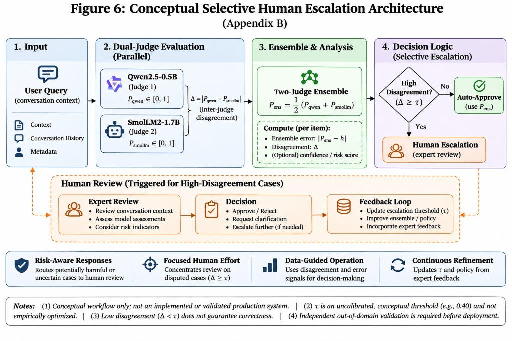
\includegraphics[width=\textwidth]{figures/fig6_escalation.pdf}
    \caption{Conceptual selective human escalation architecture (Appendix~B). Incoming user queries are evaluated in parallel by two local sub-2B open-weight judges on consumer hardware ($<1.2\text{ GB}$ RSS). In the low-disagreement regime ($\Delta < \tau$), conversations proceed with automated unweighted ensemble scoring ($P_{\text{ens}}$). In the high-disagreement regime ($\Delta \ge \tau$), cases are escalated to human expert review. \textbf{Critical Constraints:} (1) This diagram depicts an exploratory conceptual proposal, not an operational or empirically validated deployment. (2) The escalation threshold $\tau$ is conceptual and uncalibrated; optimal operational thresholds require empirical risk-utility calibration on independent out-of-domain data. (3) Low disagreement ($\Delta < \tau$) does not guarantee model correctness due to potential shared inductive biases or common failure modes.}
    \label{fig:escalation_workflow}
\end{figure*}

\subsection{Architectural Stages and Decision Logic}
\begin{enumerate}
    \item \textbf{Stage 1 (Local Input Ingestion):} Conversational turns and dialogue context are ingested without cloud API dependencies.
    \item \textbf{Stage 2 (Parallel Dual-Judge Evaluation):} \texttt{Qwen2.5-0.5B-Instruct} and \texttt{SmolLM2-1.7B-Instruct} evaluate the dialogue in parallel on commodity CPU hardware, extracting conditional unsafe continuation probabilities ($P_{\text{qwen}}$ and $P_{\text{smollm}}$).
    \item \textbf{Stage 3 (Ensemble Aggregation and Diagnostic Extraction):} The system computes the unweighted ensemble estimate $P_{\text{ens}} = \frac{1}{2}(P_{\text{qwen}} + P_{\text{smollm}})$ and inter-judge disagreement $\Delta = |P_{\text{qwen}} - P_{\text{smollm}}|$.
    \item \textbf{Stage 4 (Selective Escalation Gate):} Conversations exhibiting low disagreement ($\Delta < \tau$) are auto-scored using $P_{\text{ens}}$. Borderline or highly contested dialogues ($\Delta \ge \tau$) trigger an escalation event, routing the full conversational context and model scores to human safety specialists.
    \item \textbf{Stage 5 (Expert Review and Continuous Calibration):} Human adjudications resolve ambiguous cases, feeding back into ongoing threshold tuning and policy refinement.
\end{enumerate}

\subsection{Operational Disclaimers and Non-Deployment Status}
We explicitly emphasize that this workflow represents an exploratory conceptual model rather than a validated production system. As established in Section~\ref{subsec:disagreement_analysis}, low disagreement does not guarantee correctness, as small open-weight judges can share common blind spots. Furthermore, setting an operational threshold $\tau$ requires empirical cost-benefit optimization on an independent validation set, balancing the organizational cost of human review against the safety liability of false negatives.


\end{document}
